% ------------------------------------------------------------------------
% ------------------------------------------------------------------------
% 
% Modelo de Trabalho Acadêmico (tese de doutorado, dissertação de mestrado e
% trabalhos monográficos em geral) baseado no ICMC (USP), em conformidade com
% a ABNT NBR 14724:2011: Informação e documentação - Trabalhos acadêmicos -
% ------

% Apresentação
% ------------------------------------------------------------------------
% ------------------------------------------------------------------------

% Opções: 
%   Qualificação          = qualificacao 
%   Curso                 = doutorado/mestrado
%   Situação do trabalho  = pre-defesa/pos-defesa (exceto para qualificação)
%   Versão para impressão = impressao
\documentclass[qualificacao, mestrado, pre-defesa]{packages/icmc}

% ---------------------------------------------------------------------------
% Pacotes Opcionais
% ---------------------------------------------------------------------------
\usepackage{rotating}           % Usado para rotacionar o texto
\usepackage[all,knot,arc,import,poly]{xy}   % Pacote para desenhos gráficos
% Este pacote pode conflitar com outros pacotes gráficos como o ``pictex''
% Então é necessário usar apenas um dos pacotes conflitantes
\newcommand{\VerbL}{0.52\textwidth}
\newcommand{\LatL}{0.42\textwidth}

\usepackage{xcolor}
\newcommand{\basg}[1]{{\color{blue}[#1]}}
\providecommand{\textcite}[1]{\citeonline{#1}}

% ---------------------------------------------------------------------------


% ---
% Informações de dados para CAPA e FOLHA DE ROSTO
% ---
% Tanto na capa quanto nas folhas de rosto apenas a primeira letra da primeira palavra (ou nomes próprios) devem estar em letra maiúscula, todas as demais devem ser em letra minúscula.
\tituloPT{ESTIMADOR AUTOMÁTICO DE PARÂMETROS PARA SÍNTESE FM POR MEIO DE REDES NEURAIS CONVOLUCIONAIS}
\tituloEN{Automatic Parameter Estimator for FM Synthesis Using Convolutional Neural Networks}
\autor[Rocha da Silva, Sergio]{Sergio Rocha da Silva}
\genero{M} % Gênero do autor (M = Masculino / F = Feminino)
\orientador[Orientador]{Prof. Dr.}{Márcio Porto Basgalupp}
%\coorientador{Prof. Dr.}{Fulano de Tal}
\curso{PPGCC}
\data{21}{04}{2026} % Data do depósito
\idioma{EN} % Idioma principal do documento (PT = português / EN = inglês)
% ---


% ---
% RESUMOS
% ---

% Resumo em PORTUGUÊS
% conter no máximo 500 palavras
% conter no mínimo 1 e no máximo 5 palavras-chave
\textoresumo[brazil]{
    A síntese FM é uma das técnicas mais renomadas de síntese sonora e, embora seja um método antigo, ainda permanece amplamente utilizada atualmente. Ela é simples, computacionalmente barata e capaz de produzir resultados de alta qualidade. No entanto, o uso bem-sucedido desse tipo de síntese de áudio apresenta um desafio significativo: a seleção dos parâmetros corretos para o sintetizador. Esse processo não é preciso, e não há um procedimento totalmente determinístico a ser seguido. Os músicos geralmente são guiados pela intuição e por um processo empírico de tentativa e erro. Para revitalizar essa técnica e aproveitar seus benefícios, o uso de modelos de CNN surge como uma opção bastante promissora, pois eles podem ajudar músicos a obter resultados convincentes, imitando instrumentos reais em pouco tempo e a baixo custo, ou até mesmo criando timbres e efeitos totalmente imprevisíveis. Dessa forma, este trabalho explora essa abordagem por meio da criação de um pipeline capaz não apenas de treinar um modelo de CNN para prever os parâmetros adequados que permitam a um sintetizador FM ressintetizar amostras de áudio originais (como instrumentos acústicos), mas também de explorar amplamente o espaço de parâmetros do sintetizador, possibilitando a reprodução de sons arbitrários dentro de suas capacidades. Os resultados obtidos até aqui indicam que a abordagem é promissora para ambos os objetivos: o modelo desenvolvido foi capaz de aproximar amostras de som não vistas anteriormente (de instrumentos reais), e as métricas de erro convergiram para valores satisfatórios mesmo ao utilizar um processo exploratório de geração de dados (um conjunto de dados sintético especificamente construído para explorar as capacidades do sintetizador FM).
    }{CNN, Síntese FM, Re-Síntese, Computação Musical, Redes Neurais}


% resumo em INGLÊS
% conter no máximo 500 palavras
% conter no mínimo 1 e no máximo 5 palavras-chave
\textoresumo[english]{
    FM synthesis is one of the most renowned techniques for sound synthesis, and although it is an old method, it remains widely used today. It is simple, computationally inexpensive, and capable of producing high-quality results. However, the successful use of this type of audio synthesis presents a significant challenge: selecting the correct parameters for the synthesizer. This process is not precise, and there is no fully deterministic procedure to follow. Musicians are usually guided by intuition and an empirical trial-and-error process. To revive this technique and leverage its benefits, the use of CNN models appears to be a very promising option, as they can help musicians achieve convincing results, imitating real instruments in a short time and at a low cost, or even creating totally unpredictable timbres and effects. Therefore, this work explores this approach by creating a pipeline capable not only of training a CNN model to predict the appropriate parameters that enable an FM synthesizer to resynthesize original audio samples (such as acoustic instruments), but also of exploring the synthesizer’s parameter space broadly, allowing it to reproduce sounds within its capabilities. The results obtained so far indicate that the approach is promising for both objectives: the developed model was able to approximate unseen sound samples (of real instruments), and the error metrics converged to satisfactory values even when using an exploratory dataset generation process (a synthetic dataset specifically constructed to explore the FM synthesizer’s capabilities).
    }{CNN, FM Synthesis, Re-Synthesis, Music Computing, Neural Networks}


% ----------------------------------------------------------
% ELEMENTOS PRÉ-TEXTUAIS
% ----------------------------------------------------------

% Inserir a ficha catalográfica
\incluifichacatalografica{tex/pre-textual/ficha-catalografica.pdf}

% DEDICATÓRIA / AGRADECIMENTO / EPÍGRAFE
\textodedicatoria*{tex/pre-textual/dedicatoria}
\textoagradecimentos*{tex/pre-textual/agradecimentos}
\textoepigrafe*{tex/pre-textual/epigrafe}

% Inclui a lista de figuras
\incluilistadefiguras

% Inclui a lista de tabelas
\incluilistadetabelas

% Inclui a lista de quadros
\incluilistadequadros

% Inclui a lista de algoritmos
\incluilistadealgoritmos

% Inclui a lista de códigos
\incluilistadecodigos

% Inclui a lista de siglas e abreviaturas
\incluilistadesiglas



% Inclui a lista de símbolos
\incluilistadesimbolos

% ----
% Início do documento
% ----
\begin{document}
% ----------------------------------------------------------
% ELEMENTOS TEXTUAIS
% ----------------------------------------------------------
\textual

\chapter{Introduction}
\label{chapter:introduction}
% Comando simples para exibir comandos Latex no texto
\newcommand{\comando}[1]{\textbf{$\backslash$#1}}

Musical expression is one of humanity’s earliest experiences and one of the most valued forms of art. This art form has been cultivated since ancient times. The Chinese, three thousand years before Christ, had already developed complex systems of musical theory, and Greek culture not only cultivated its study but also associated it with their cults, attributing idols characteristics to protect and honor music itself \textcite{med1996teoria}.

Although music is a subjective form of human knowledge, the recorded music industry today moves approximately US\$29 billion per year \textcite{ifpi2025}, and thus its value is no longer only subjective.

It is precisely in this context that synthesized sound appears in history. It emerged after the first electronic instruments and, due to the periodic nature of sound, the earliest synthesizers were composed of simple analog oscillators that could be manually controlled through operations such as summing and filtering \textcite{holmes2016electronic}.

In the 1980s, with the release of the Yamaha DX7 synthesizer, the history of music synthesis took a major turn. The Yamaha DX7 marked the first major success of a revolutionary technique developed by John M. Chowning at Stanford University and later popularized by Yamaha \textcite{claesson2021resynthesis}. This event represented a new milestone in sound synthesis, not only because of its popularity, but also because it made the reproduction of both realistic instrument simulations and entirely new kinds of sounds accessible to musicians and composers of all levels. In fact, FM synthesis was so successful that the technique remains in use to this day \textcite{holmes2016electronic}.

This long-standing relevance is especially important because, despite the emergence of newer approaches such as wavetable synthesis, sample-based methods, and GAN-based sound generation, FM synthesis continues to occupy an important place in the contemporary musical ecosystem. Each of these alternatives has strengths and limitations: sample-based methods can be difficult to design and are limited in their ability to generate genuinely new timbres, while GAN-based approaches can produce highly realistic results but often require substantial computational resources. By contrast, FM synthesis remains attractive because it is relatively accessible, flexible, well suited for experimenting with new and even unpredictable sounds, and adaptable to real-time composition.

Thus, the primary goal of the present work is to guide a synthesizer based on frequency modulation (FM) to reproduce instrument sound samples, while also developing a process that explores the expressive capabilities of the FM synthesizer itself and aims at approximating the resynthesis of arbitrary input sounds within the system's capabilities.

This approach aligns with one of the key historical advantages of FM synthesizers: their ability to create sounds that cannot be produced by traditional acoustic instruments.

Within this context, researchers continue to focus on improving the control of traditional FM synthesis parameters, which, when done manually, can be a tedious empirical process. For instance, \textcite{claesson2021resynthesis} implemented a neural network to predict FM synthesizer parameters using frequency-domain sound representations as input. Similarly, \textcite{steinmetz2022ddx7} proposed a TCN-based approach that couples the FM synthesizer directly within the network training process.

The present work, however, employs a Convolutional Neural Network (CNN) to achieve its goals, because CNNs enable the direct use of raw audio samples as model input while also serving as effective feature extractors for sound signals \textcite{kiranyaz2021survey}. CNNs are also well known for their ability to economize computational resources when handling high-dimensional data, which makes them a strong candidate for this type of research task.

Furthermore, beyond a simple resynthesis exercise, this work aims to develop a process that allows the model to achieve a broad understanding of the entire parameter space of the applied FM synthesizer. The idea behind the proposed methodology is that, if the model can learn the FM synthesizer’s parameter space in a comprehensive way, it can then be used to simulate any sound within the synthesizer’s capabilities, making the experience of a future user, such as a musician or composer, much more efficient in achieving the desired sound and integrating it into real composition workflows.

Therefore, this work aims not only to apply a machine learning technique, but also to propose an approach that may be adapted to different FM synthesizers, potentially providing practical utility for users interested in sound design and music production.

The remainder of this thesis is organized as follows. Chapter~\ref{chapter:theoretical_basis} discusses the fundamental concepts needed to understand and apply the techniques used in this research. Chapter~\ref{chapter:related_works} reviews the related work. Chapter~\ref{chapter:methodology} describes the proposed approach and the experimental setup. Chapter~\ref{chapter:experimental_results} presents and analyzes the results. Finally, Chapter~\ref{chapter:conclusion} provides the conclusions of this work and outlines directions for future research.


\chapter{Related Works}
\label{chapter:related_works}
Several studies have explored machine learning approaches for estimating parameters of sound synthesizers. The central choice in this work is to use Convolutional Neural Networks (CNNs) directly on raw audio signals. This choice is motivated by three practical aspects: raw waveforms preserve temporal structure, CNNs are well suited to high-dimensional inputs, and once trained they can provide fast inference. In addition, as emphasized by the ``Bitter Lesson'', greater reliance on data and computation often outperforms approaches based on hand-crafted representations~\cite{sutton2019bitterlesson}. In this sense, the present work follows a data-driven perspective in which the model learns the relevant patterns directly from the signal, without relying on a manual feature pipeline.

Claesson et al.~\cite{claesson2021resynthesis} proposed the re-synthesis of instrumental sounds using machine learning models combined with an FM synthesizer. Their approach, however, used STFT spectrograms as input rather than raw audio. Although this frequency-domain representation may simplify learning, it also introduces an additional preprocessing stage and does not fully exploit the temporal information present in the waveform. Steinmetz et al.~\cite{steinmetz2022ddx7} introduced DDX7, a differentiable FM synthesizer designed for musical instrument re-synthesis. Their method employs a Temporal Convolutional Network (TCN) and integrates Mel-spectrum losses, which provides a perceptually aligned training objective. The main trade-off is that the synthesizer must be embedded in the training loop, increasing computational and memory cost.

Finally, Kiranyaz et al.~\cite{kiranyaz2021survey} presented a comprehensive survey on one-dimensional CNNs and their applications, highlighting their effectiveness for sequential data such as audio signals. This survey supports the suitability of CNN-based architectures for learning temporal patterns directly from raw audio. In contrast to the works above, the present study emphasizes generalization through large-scale randomized exploration of the FM parameter space, while keeping the synthesizer outside the optimization process. This also makes the resulting model suitable for fast inference after training, which is important for interactive and real-time-oriented audio applications.


\chapter{Theoretical Basis}
\label{chapter:theoretical_basis}
This chapter introduces the theoretical fundamentals underlying this research. Although these concepts will be presented with an introductory approach, a basic understanding of Machine Learning and Neural Networks is expected. However, this section will cover Musical Computation, FM Synthesis, Fourier Transform, Neural Networks, and One Dimensional Convolutional Neural Networks.

\section{Musical Computation}

Musical computation is a broad and interdisciplinary field that encompasses all aspects of musical processing through a computer. It is beyond the scope of this thesis to provide a comprehensive overview of this field; however, for the purposes of this study, it is important to cover the basic elements of sound and the fundamentals of audio digitization.

\subsection{Sound elements}

Audio is a mechanical compression wave that travels through the air. This type of wave can be converted into an electrical signal through microphones, which consist of an arrangement of coils and magnets. As a wave, its main elements are:

\begin{itemize}
\item Pitch: The fundamental frequency of a sound, which determines whether it is low or high. The higher the frequency, the higher the pitch.
\item Duration: The length of time a sound is sustained and can be heard.
\item Loudness (or amplitude): The intensity or energy level of a sound. In terms of a wave, it corresponds to the amplitude of the sound wave.
\item Timbre: Like the color of a visual object, timbre refers to the quality or "color" of a sound. This aspect will be treated in more detail in the next section.
\end{itemize}

It is important to highlight that although sound can be described in terms of the aspects mentioned above, hearing is mainly a cognitive process. Therefore, sound comparison cannot be fully addressed by mathematical tools, leaving a significant space for perceptual comparison and classification (not to mention aspects related to personal preferences).

\subsubsection{Sound timbre}

Another important aspect of acoustic sounds is timbre, which can be understood as the “color of sound.”

From a mathematical point of view, timbre varies according to the harmonics present in a sound sample, or, in other words, according to the set of oscillations that compose the sound.

In the case of acoustic instruments, what happens is that the air vibrations produced by the instrument are not simple pure sinusoids. In fact, when a string vibrates, or when air resonates inside a tube, many parts of the instrument's body vibrate simultaneously, and the frequency with which each part vibrates differs according to its composition, position, and other factors. The result is that each instrument has a unique sound, especially in the case of handcrafted wooden instruments such as violins or cellos.

To obtain a clear visualization of this aspect, it is common to convert a sound sample from the time domain to the frequency domain using a Fourier Transform technique.

For example, consider the image~\ref{fig:time_domain_violin} which presents violin audio sample in time domain, and the image \ref{fig:frequency_domain_violin} which presents the same audio, but in frequency domains.

\begin{figure}[h]
    \centering
    
\includegraphics[width=\linewidth]{../images/time_domain_violin.png}
    \caption{One second time domain violin sample.}
    \label{fig:time_domain_violin}
\end{figure}

\begin{figure}[h]
    \centering
    
\includegraphics[width=\linewidth]{../images/frequency_domain_violin.png}
    \caption{The same one second frequency domain violin sample.}
    \label{fig:frequency_domain_violin}
\end{figure}

As the figures show, there is a main frequency that defines the pitch of the sound, along with many other frequencies that allow the ear to identify the instrument and distinguish between different kinds of sounds.

\subsection{Audio digitalization}

A microphone converts a pressure wave into an electrical waveform. However, in computational music, the audio signal must be discretized to be represented as a digital audio file. The primary process for digital audio representation is sampling.

Sampling consists of recording a sequence of wave amplitudes at fixed intervals. For example, if a sound is recorded using a sampling rate of 22,100 Hz, it means that the computer will capture 22,100 audio samples per second.

\begin{figure}[htb]
 \caption{Signal sampling}
 \label{fig:signal_sampling}
 \centering
 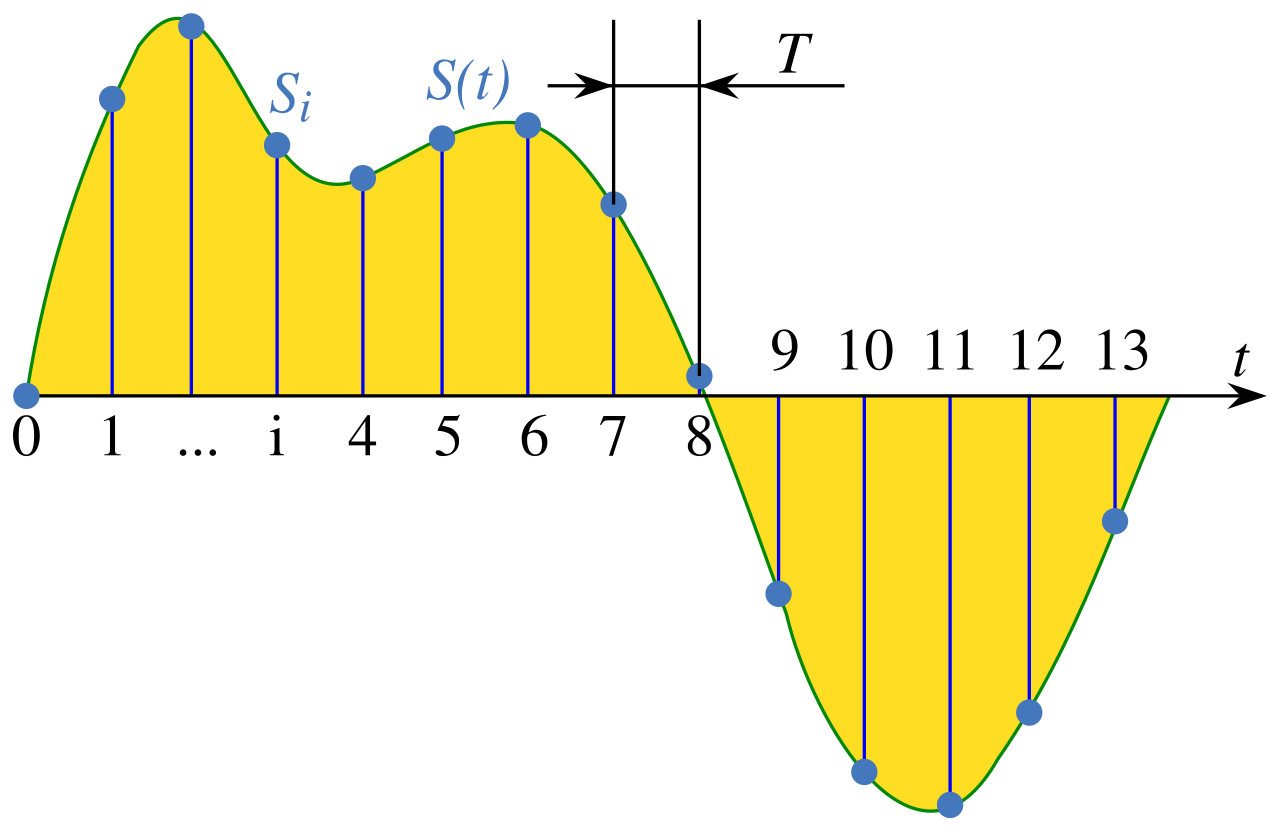
\includegraphics[scale=0.2]{images/signal_sampling.png}
 \fdireta{usp:logo}
\end{figure}

This approach is very efficient because human hearing can detect frequencies between 20 Hz and 20,000 Hz. However, for most musical sounds, the maximum frequency is typically below 10 kHz (in fact, even a violin—one of the highest-pitched instruments—reaches only around 3,500 Hz). And according to the Nyquist-Shannon Theorem, to properly sample a periodic signal, the sampling rate must be at least twice the frequency of the highest component of the signal.

Thus, 22,100 Hz can be a good sampling rate for recording music while saving disk space. However, if the goal is to cover the full range of human hearing, higher rates, such as 44,200 Hz, can also be used.

Note that with this process, all sound elements highlighted before, can be recorded and reprocedure later.

\subsection{Sound synthesis}

After the development of sound recording techniques, musical computation evolved toward the creation of artificial waveforms. Of course, before digital audio synthesis, there were several techniques that allowed analog synthesis. However, the underlying idea is essentially quite similar.

In summary, audio synthesis techniques can be divided into three basic types:

\begin{itemize}
\item \textbf{Additive synthesis:} Perhaps the most straightforward idea from a mathematical point of view. It consists of generating each frequency component of a desired timbre separately and then summing them. In fact, it is more like a weighted sum, since each component is weighted according to its contribution to the timbre. A normalization step is commonly applied after the process to avoid amplitude overload.

\item \textbf{Subtractive synthesis:} The opposite of the previous technique, but historically more common due to its effectivenessa and lower cost. In short, it consists of taking a complex waveform, rich in harmonics, and applying various filters to obtain the desired sound. It is more empirical than additive synthesis (which is based on spectral analysis), but simpler to implement and less computationally intensive. Typically, the original waveforms are complex ones such as the sawtooth wave, square wave, or triangular wave.

\item \textbf{FM synthesis:} Another empirical approach to sound synthesis, which will be addressed in detail in a later section. In short, it consists of altering a simple waveform by applying a high-frequency modulation, not to the generated waveform itself, but directly to the frequency parameter of the carrier oscillator. This kind of distortion of the base frequency produces mirrored harmonics that enrich the timbre of the sound. It is up to the musician to choose the appropriate parameters to produce the desired timbre.
\end{itemize}

There are many other techniques that could be mentioned; however, these three represent the most direct forms of synthesis, or the most purely mathematical ones, in the sense that they do not require manipulation of pre-recorded audio.

\subsubsection{ADSR Audio envelop}

Another important technique for achieving good results is the so-called “Attack, Decay, Sustain, and Release (ADSR) envelope”, which consists of applying a multiplicative function to the waveform, altering only its amplitude.

The basic idea is to control the sound intensity by simulating the natural behavior of acoustic sounds. Typically, an ADSR envelope is defined as a function with a domain between 0 and 1, which is applied to the generated waveform:

\begin{figure}[h]
    \centering
    
\includegraphics[width=\linewidth]{../images/adsr.png}
    \caption{ADSR linear envelop.}
    \label{fig:adsr_linear_envelop}
\end{figure}

The ADSR envelope can be understood as an amplitude function:

\[
y(t) = e(t) \cdot s(t)
\]

Where:

\begin{itemize}
\item \( s(t) \): the raw generated sound wave.
\item \( e(t) \): the ADSR envelope function (normalized amplitude ranging from 0 to 1).
\item \( y(t) \): the resulting sound.
\end{itemize}

Although real audio samples can show a wide variation of envelope behaviors, it is common practice to use a linear function to achieve the goal, since the human ear is more sensitive to abrupt changes and to relative differences. However, for long time variations, the ear can still perceive the change, which is why some synthesizers allow the use of exponential or logarithmic functions as well.

\subsection{FM Synthesis}

As shown in the previous sections, one of the most popular sound synthesis techniques is Frequency Modulation Synthesis (FM Synthesis), which was introduced by John M. Chowning in his famous paper “The Synthesis of Complex Audio Spectra by Means of Frequency Modulation”, published at the Stanford Artificial Intelligence Laboratory.

Chowning explored the effects of frequency modulation when applied with high frequencies, close to the audible range, instead of the traditional use of inaudible frequencies.

In fact, the concept of frequency modulation was already well known before this paper; however, it had been used mainly in radio transmission of music or to apply slight distortions through low-frequency oscillators (LFOs), producing effects such as vibrato.

As Chowning himself pointed out in his paper, when the technique is applied to vary the frequency of the carrier wave through a high-frequency modulator wave, it “results in a surprising control of audio spectra” (\cite{chowning1973synthesis}).

In summary, considering only two oscillators: the main one, called the carrier, and the modulator, so the instantaneous frequency of the output audio can be expressed by the following function:

\[
f(t) = f_c + I \cdot \sin(2\pi f_m t)
\]

Where:

\begin{itemize}
\item \( f(t) \): the instantaneous frequency of the generated sound wave.
\item \( f_c \): the original frequency of the carrier wave.
\item \( I \): the modulation index, which defines the intensity of the modulation (the greater the value, the more harmonics are generated).
\item \( f_m \): the frequency of the modulator wave (which determines the spacing of the harmonics).
\item \( t \): the time variable.
\end{itemize}

The most important point, however, is that this simple manipulation results in symmetric sidebands around the carrier frequency, spaced at multiples of \( f_m \).

For a more intuitive understanding, if a carrier frequency \( f_m \) is modulated by a frequency \( f_m \), the resulting spectrum will contain:

\[
f_c \pm n f_m
\]

For example, by choosing \( f_c = 440 \) and \( f_m = 220 \), the resulting wave will contain frequency components such as 220 Hz, 440 Hz, 660 Hz, 880 Hz, and so on, with decreasing amplitudes (the amplitudes follow the Bessel coefficients, but this discussion is beyond the scope of this article).

The last important characteristic of Frequency Modulation Synthesis concerns the ratio between the carrier frequency and the modulator frequency \( f_c / f_m \), since this ratio directly influences the perceived audio result.

This ratio determines whether the generated harmonics align with the natural harmonic series (widely used by musicians) or not:

\begin{itemize}
    \item If the ratio is an integer number, the harmonic sidebands (in the spectral view) will appear as integer multiples of \( f_c \), generating harmonic sounds similar to those of real instruments (consistent with traditional music theory).
    \item If the ratio is not an integer value, the harmonic sidebands will not align perfectly with \( f_c \), and the generated sound may appear metallic or dissonant (but, this effect is useful for creating sounds such as bells or for producing special audio effects).
\end{itemize}

\subsection{Audio comparison}

The task of audio comparison is not straightforward, especially when the goal is to achieve equality in terms of human perception. It can be complex, computationally demanding, and inherently subjective.

However, as described in the section on timbre, one intuitive and efficient way to approach this problem is by comparing the audio in its spectral representation, since timbre is precisely defined by this combination of frequencies.

That said, this approach alone is not sufficient, because the Fourier Transform considers the entire audio signal at once, mixing different parts of a sound sample. For example, if a sample contains three different pitches in sequence, its frequency-domain representation will show them simultaneously, which may give the impression that the timbre is a mixture of all these pitches (similar to a chord rather than a sequence).

In fact, according to \cite{claesson2021resynthesis}, FFT-based spectral comparison is valid but only a part of the solution. He highlights the following metrics:

\begin{itemize}
    \item \textbf{FFT Distance:} This metric consists of computing the Fast Fourier Transform (FFT) of the two samples being compared and then calculating the Euclidean distance between them. The result can be normalized so that the maximum distance is 1 and the minimum is 0.
    \item \textbf{Short Time Fourier Transform (STFT) Distance:} Equivalent to the FFT Distance, but calculated over short, overlapping slices of the sample, which provides time-localized spectral information.
    \item \textbf{Log-Mel Spectogram Distance:} Similar to the previous metrics, but based on the Log-Mel Spectrogram, which is essentially an adaptation of the FFT spectrum that incorporates human auditory perception. In summary, the Log-Mel Spectrogram is obtained by computing the STFT, mapping the frequencies onto the Mel scale (explained later in this document), and finally projecting the amplitudes onto a logarithmic scale.
\end{itemize}

In addition to these three metrics, \cite{claesson2021resynthesis} also recommends the use of Euclidean Distance of the Envelope to compare audio envelopes. This approach can be very useful, but since this work is focused on the similarity between original and synthesized audio in terms of timbre, the envelope comparison, while important for real-world applications, falls outside the scope of the present study.

\subsubsection{Mel-Scale Representation}

The Mel scale was proposed by Stevens, Volkmann, and Newman in 1937 (\cite{claesson2021resynthesis}), and its main purpose is to reflect the human perception of frequency.

The key difference from the linear scale is that, as the values on the scale increase, the perceptual difference between two adjacent points becomes smaller.

In fact, the Mel scale maps linear frequencies onto a logarithmic scale. A frequency \( f \) s converted to the Mel scale through the following formula:

\[
\text{Mel}(f) = 2595 \log_{10} \left( 1 + \frac{f}{700} \right)
\]

For a better understanding of this conversion, consider the following graph, which compares the linear hertz scale with the Mel scale:

\begin{figure}[h]
    \centering
    
\includegraphics[width=\linewidth]{../images/mel_scale.png}
    \caption{Comparision between linear hertz scale and Mel scale (\cite{claesson2021resynthesis}).}
    \label{fig:mel_scale_comparison}
\end{figure}

It is a very useful metric for audio comparison, as it takes into account the human auditory perception of frequency.

\section{1D Convolutional Neural Networks}

\subsection{History and motivation}

Convolutional Neural Networks (CNNs) originated in the 1990s with the introduction of the "LeNet" model. Since their inception, CNNs have demonstrated remarkable results in classification tasks.

Although this type of neural network went through a period of relative stagnation—due to the rise of alternative machine learning paradigms such as Support Vector Machines and Bayesian Networks—CNNs eventually became the de facto standard for computer vision problems, including object detection, image classification, and other image-based machine learning challenges.

The significant breakthrough in the use of CNNs can be attributed to two main factors: (1) the simplicity with which CNNs handle input data, such as images; and (2) the efficient use of computational resources during training.

Regarding simplicity, since the advent of CNNs, many image-based machine learning tasks no longer require extensive pre-processing before applying learning algorithms to solve the target problem.

For example, consider the problem of bird species classification based on images. In such a task, it is easy to observe that for many species, simple color patterns (e.g., on the bird's plumage) may be sufficient for identification. For other species, the analysis of connected components in the image—such as textures and visual patterns—can play a crucial role. Furthermore, in other cases, the frequency of color variations across the image may serve as a key classification feature.

Therefore, different filters are required to detect distinct properties in the images, making it possible to apply machine learning techniques—such as decision trees—for effective image classification.

In addition, several other important factors must be considered to improve classification performance, including image rotation, scale variation, translation, lighting conditions, and more.


\chapter{Methodology}
\label{chapter:methodology}
This chapter describes the methodology adopted to achieve the project goals. It summarizes the main steps, details the implementation choices, and specifies the experimental protocol so the study can be reproduced.

\section{General Idea}

The project aims to use AI to guide an FM synthesizer to simulate any target timbre. In practical terms, a CNN receives a raw audio sample and predicts a set of FM parameters that can re-synthesize the same sound, allowing the synthesizer to emulate an instrument playing musical sounds (or even emulate not musical sounds).

To operationalize this idea, the methodology follows the steps below:

\begin{enumerate}
  \item Implement a simple FM synthesizer suitable for controlled data generation and evaluation.
  \item Generate a synthetic dataset of audio samples and corresponding parameter values.
  \item Train a CNN regressor to predict synthesizer parameters from raw audio.
  \item Evaluate generalization using the Google NSynth dataset and objective audio similarity metrics.
\end{enumerate}

FM synthesis was selected because it offers expressive timbral control at low computational cost, yet requires expert knowledge to tune. Then, learning parameter mappings with a neural model reduces manual effort (of a trial-and-error process) while enables fast and repeatable synthesis.

All experiments were conducted on the following software and hardware environment:

\begin{itemize}
  \item Python 3.11.2
  \item TensorFlow 2.19.0
  \item Keras 3.11.1
  \item NVIDIA CUDA 12.5.82
  \item cuDNN 3.0.75
  \item NVIDIA driver 535.247.01
  \item CUDA toolkit 12.2
  \item NVIDIA GeForce GTX 1650 GPU with 4 GB of memory
\end{itemize}

\section{Implementing the FM Synthesizer}
\label{sec:fm_synth}

There are several commercial FM synthesizers with hundreds or thousands of parameters. However, this work focuses on a research-oriented, controllable baseline. Therefore, a deliberately simple synthesizer was implemented to validate the overall pipeline.

Commercial synthesizers can expose extremely large parameter spaces. For example, Native Instruments' FM8 can use around 1,000 parameters, while the Teenage Engineering OP-1 has been described as reaching up to $10^{76}$ possible parameter combinations \cite{claesson2021resynthesis}. These figures reinforce why a simplified synthesizer is useful in this study: it keeps the experimentation tractable while still exercising the main FM synthesis concepts.

\begin{figure}[h]
  \centering
  
\includegraphics[width=0.9\linewidth]{../images/first_part.png}
  \caption{Overview of the synthesis implementation.}
  \label{fig:met1}
\end{figure}

The implemented synthesizer uses 6 (six) operators inspired by the Yamaha DX7 and supports two algorithms (one fully serial and one mixed serial/parallel). It contains 5 modulator operators, 1 carrier operator, and a single ADSR envelope. The two operator topologies are shown in Figure~\ref{fig:FMSynth}.

\begin{figure}[h]
  \centering
  
\includegraphics[width=0.85\linewidth]{../images/algs2.png}
  \caption{FM synthesizer operator algorithms.}
  \label{fig:FMSynth}
\end{figure}

The synthesis pipeline follows four steps:

\begin{enumerate}
  \item Generate each operator signal by phase modulation of the next operator in the chain.
  \item Combine operator outputs according to the selected algorithm (parallel outputs are summed).
  \item Apply the ADSR envelope.
  \item Downsample from 48 kHz to 16 kHz with a low-pass filter to avoid aliasing.
\end{enumerate}

A 48 kHz internal rate was used to reduce aliasing caused by high-frequency components generated by FM operators. Downsampling is performed with low-pass filtering to maintain stability and avoid wrong spectral artifacts.

The synthesizer exposes 16 parameters: 12 parameters for ratios and modulation indices (beta) across the five modulators and the carrier, plus 4 ADSR parameters (attack, decay, sustain, release). This configuration is intentionally minimal yet sufficient to cover the FM principles needed for the study.

\section{Datasets}
\label{sec:datasets}

Two datasets are used: a synthetic dataset for training and a real-instrument dataset (NSynth) for evaluation.

\subsection{Synthetic dataset}

The synthetic dataset is built by sampling FM parameters and rendering the corresponding audio. This produces explicit tuples of (parameters, audio), enabling supervised training of the CNN/regressor. The parameter sampling strategy follows prior FM resynthesis work that constrains the search space to musically plausible ranges while still exploring diverse timbres \cite{claesson2021resynthesis}.

\begin{figure}[h]
  \centering
  
\includegraphics[width=0.9\linewidth]{../images/second_part.png}
  \caption{Synthetic dataset generation overview.}
  \label{fig:met2}
\end{figure}

Each sample is 4 seconds long, monophonic, and stored at 16 kHz (signals are generated at 48 kHz and then downsampled for compatibility with NSynth dataset). The dataset contains 5,000 samples, with pitches between 20 Hz and 6 kHz and randomized ADSR envelopes.

To make the random samples musically plausible and reduce aliasing, the following constraints were applied:

\begin{itemize}
  \item Carrier frequency is drawn uniformly from 20 Hz to 6 kHz, keeping the highest base frequencies below the Nyquist limit after downsampling.
  \item Modulator ratios are constrained to the range [1/8, 8]. With 90\% probability the ratio is drawn from a discrete harmonic-like set; with 10\% probability it is drawn from a log-uniform distribution to allow metallic timbres \cite{chowning1973synthesis,nielsen2020practical}.
  \item Modulation indices (beta) are drawn uniformly in [0, 8] with a biased distribution: 20\% in [0, 0.5], 60\% in [0.5, 3], and 20\% in [3, 8], prioritizing rich but stable timbres and increasing sideband count and spectral bandwidth as the index grows \cite{chowning1973synthesis,nielsen2020practical}.
  \item Amplitude is fixed at 1.0 to avoid parameter redundancies that yield identical spectra.
  \item ADSR parameters are sampled from uniform intervals: attack in [0.005, 0.5] s, decay in [0.02, 0.6] s, sustain in [0.1, 0.9], and release in [0.05, 0.8] s.
\end{itemize}

The dataset is split into 3,750 training samples and 1,250 test samples. From the training split, 20\% is reserved for validation, resulting in 3,000 training and 750 validation samples.

\subsection{External dataset (NSynth)}

The NSynth dataset from Google Magenta project contains real instrument samples and is used to evaluate generalization \cite{engel2017nsynth}. Only the test subset is used during evaluation, with:

\begin{itemize}
  \item 4,096 samples;
  \item 4 seconds per sample;
  \item 16 kHz sampling rate;
  \item 11 instrument families;
  \item pitches from 27.5 Hz to 4,186.01 Hz.
\end{itemize}

\section{Training the CNN}
\label{sec:training_cnn}

The mapping from audio to FM parameters is not analytically tractable, because each operator introduces additional spectral components. Therefore, this work learns the mapping from raw waveforms using a CNN-based regressor.

\begin{figure}[h]
  \centering
  
\includegraphics[width=0.9\linewidth]{../images/thrid_part.png}
  \caption{Model training and optimization overview.}
  \label{fig:met3}
\end{figure}

\subsection{Model architecture}

The model combines a CNN-based feature extractor with a fully connected regressor. Figure~\ref{fig:redes} summarizes the two modules.

\begin{figure}[h]
  \centering
  \begin{subfigure}[b]{0.45\textwidth}
    \centering
    
\includegraphics[width=\textwidth,height=0.4\textwidth,trim={0 0 0 0.6cm},clip]{../images/rede1.png}
    \caption{Feature extraction}
    \label{fig:rede1}
  \end{subfigure}
  \hfill
  \begin{subfigure}[b]{0.45\textwidth}
    \centering
    
\includegraphics[width=\textwidth,height=0.4\textwidth,trim={0 0 0 0.85cm},clip]{../images/rede2.png}
    \caption{Regressor}
    \label{fig:rede2}
  \end{subfigure}
  \caption{Overview of the CNN feature extractor and regressor.}
  \label{fig:redes}
\end{figure}

The CNN uses three Conv1D–MaxPooling blocks, while the regressor uses two dense layers and a linear output. The hyperparameters are summarized in Tables~\ref{tab:hyperparams_cnn} and \ref{tab:hyperparams_regressor}.

\begin{table}[htb] \small \centering
  \caption{Hyperparameters of the CNN feature extractor}
  \label{tab:hyperparams_cnn}
  \begin{tabular}{l|l|l}
    \hline
    Component        & Hyperparameter            & Value       \\
    \hline
    Conv1D (1)       & Filters / Kernel / Stride & 8 / 4 / 1   \\
    MaxPooling1D (1) & Pool size                 & 16          \\
    Conv1D (2)       & Filters / Kernel / Stride & 16 / 8 / 1  \\
    MaxPooling1D (2) & Pool size                 & 16          \\
    Conv1D (3)       & Filters / Kernel / Stride & 32 / 16 / 1 \\
    MaxPooling1D (3) & Pool size                 & 16          \\
    \hline
  \end{tabular}
\end{table}

\begin{table}[htb] \small \centering
  \caption{Hyperparameters of the regressor network}
  \label{tab:hyperparams_regressor}
  \begin{tabular}{l|l|l}
    \hline
    Component      & Hyperparameter & Value  \\
    \hline
    Dense (1)      & Activation     & ReLU   \\
    Dropout        & Rate           & 0.5    \\
    Dense (2)      & Activation     & ReLU   \\
    Dense (Output) & Activation     & Linear \\
    Optimizer      & --             & Nadam  \\
    \hline
  \end{tabular}
\end{table}

Additional settings include:

\begin{itemize}
  \item target normalization (zero mean and unit variance);
  \item MSE as loss;
  \item MAE/MSE as metrics;
  \item batch size 32;
  \item early stopping with patience 20 and best-weight restoration;
  \item training ran for up to 200 epochs;
\end{itemize}

\subsection{Hyperparameter optimization}

A randomized grid search was used to explore a broad hyperparameter space without exhaustive testing. Table~\ref{tab:hyperparams_options} lists the options. The full grid contains 5,184 combinations; 186 experiments (about 3.6\%) were sampled, each trained for 30 epochs with early stopping (patience 5). MLflow was used to track metrics and compare configurations.

\begin{table}[htb] \small \centering
  \caption{Hyperparameter options used in randomized search}
  \label{tab:hyperparams_options}
  \begin{tabular}{l|l}
    \hline
    Hyperparameter               & Options                                      \\
    \hline
    Activation                   & gelu, swish, elu, relu, selu, silu           \\
    CNN bias                     & true, false                                  \\
    CNN kernel regularizer       & none, l1, l2                                 \\
    Regressor bias               & true, false                                  \\
    Regressor dropout            & 0, 0.2, 0.3, 0.5                             \\
    Regressor kernel regularizer & none, l1, l2                                 \\
    Optimizer                    & AdamW, RMSprop, Adam, Nadam, Adagrad, Adamax \\
    \hline
  \end{tabular}
\end{table}

\begin{figure}[h]
  \centering
  
\includegraphics[width=\linewidth]{../images/graph_grid_search.png}
  \caption{MLflow grid search results for the sampled configurations.}
  \label{fig:graph}
\end{figure}

\section{Evaluation Method}
\label{sec:evaluation_method}

The NSynth test subset is used to evaluate generalization. Each NSynth sample is passed through the CNN to predict parameters, which are then applied to the synthesizer to re-synthesize the signal. The original and re-synthesized signals are compared with objective metrics.

\begin{figure}[h]
  \centering
  
\includegraphics[width=0.9\linewidth]{../images/fourth_part.png}
  \caption{Evaluation workflow used for generalization testing.}
  \label{fig:met4}
\end{figure}

The evaluation uses FFT distance, STFT distance, and Log-Mel distance (raw and normalized). Before synthesis, ratio parameters are rounded to the nearest discrete harmonic values (matching the synthetic dataset), and parameters are clipped to the same bounds used in training. As a baseline, the same metrics are computed between each NSynth sample and a pure sinusoid at 440 Hz (A4).


\chapter{Experimental Results and Discussion}
\label{chapter:experimental_results}
This chapter reports the experimental outcomes for both training performance on the synthetic dataset and generalization to real instruments using NSynth. The results are grouped into training behavior, parameter prediction accuracy, and audio similarity metrics.

\section{Training Results}

Table~\ref{tab:train_val_metrics_2} summarizes the last five epochs of training, showing stable convergence and no signs of overfitting. Figure~\ref{fig:mae_mse_evolution} illustrates the evolution of MAE and MSE across epochs.

\begin{table}[htb]
  \centering
  \small
  \caption{Training and validation metrics by epoch.}
  \label{tab:train_val_metrics_2}
  \begin{tabular}{c|ccc|ccc}
    \hline
    Epoch & \multicolumn{3}{c|}{Train} & \multicolumn{3}{c}{Validation} \\
     & Loss & MAE & MSE & Loss & MAE & MSE \\
    \hline
    70 & 0.603 & 0.527 & 0.545 & 0.622 & 0.517 & 0.562 \\
    71 & 0.601 & 0.526 & 0.542 & 0.637 & 0.520 & 0.569 \\
    72 & 0.605 & 0.526 & 0.545 & 0.621 & 0.516 & 0.565 \\
    73 & 0.602 & 0.524 & 0.541 & 0.625 & 0.522 & 0.568 \\
    74 & 0.611 & 0.528 & 0.548 & 0.625 & 0.520 & 0.563 \\
    \hline
  \end{tabular}
\end{table}

\begin{figure}[h]
    \centering
    
\includegraphics[width=\linewidth]{../images/mae_mse_evolution.png}
    \caption{Evolution of MAE and MSE during training.}
    \label{fig:mae_mse_evolution}
\end{figure}

After training, a held-out synthetic split was used to compute test errors in the original parameter space. The results were:

\begin{itemize}
\item Mean Absolute Error (MAE): 6.488
\item Mean Squared Error (MSE): 1410.097
\item Root Mean Squared Error (RMSE): 37.551
\end{itemize}

\section{Audio Comparison Results}

Generalization was evaluated by re-synthesizing the NSynth test set and comparing the generated audio against the original recordings. A baseline comparison was computed using a pure 440 Hz sinusoid. Table~\ref{tab:metrics} shows mean and standard deviation values, and the improvement is defined as \((\text{baseline} - \text{resynthesis}) / \text{baseline}\).

\begin{table}[htb]
  \centering
  \small
  \caption{Resynthesis vs. baseline with improvement (mean and standard deviation in parentheses).}
  \label{tab:metrics}
  \begin{tabular}{l|c|c|c|c}
    \hline
    & FFT & STFT & Log Mel (raw) & Log Mel (normalized) \\
    \hline
    Resynthesis & 12649.9 (6208.1) & 2366.4 (1132.2) & 138.73 (47.013) & 0.0086 (0.0029) \\
    Baseline & 33508.8 (1887.36) & 7290.4 (434.87) & 184.87 (30.136) & 0.0115 (0.0019) \\
    Improvement (\%) & 62.250 & 67.540 & 24.960 & 24.930 \\
    \hline
  \end{tabular}
\end{table}

To analyze behavior across timbral families, metrics were aggregated by instrument group. Table~\ref{tab:avg_metrics_groups} presents the average values. The best results were obtained for keyboard, guitar, and mallet families, while vocal and organ were the most challenging.

\begin{table}[htb]
  \centering
  \small
  \caption{Average values by instrument group.}
  \label{tab:avg_metrics_groups}
  \begin{tabular}{l|c|c|c|c}
    \hline
    Group & FFT & STFT & Log Mel (raw) & Log Mel (normalized) \\
    \hline
    bass     & 11232.7 & 2144.32 & 135.610 & 0.00841 \\
    brass    & 14371.1 & 2682.95 & 167.617 & 0.01039 \\
    flute    & 14611.3 & 2872.69 & 141.819 & 0.00879 \\
    guitar   & 9692.0  & 1867.47 & 119.853 & 0.00743 \\
    keyboard & 9619.3  & 1772.92 & 119.529 & 0.00741 \\
    mallet   & 8085.8  & 1632.45 & 120.610 & 0.00748 \\
    organ    & 18360.1 & 3453.13 & 166.433 & 0.01032 \\
    reed     & 12740.0 & 2267.08 & 140.701 & 0.00872 \\
    string   & 12883.7 & 2390.65 & 139.365 & 0.00864 \\
    vocal    & 31028.9 & 5271.26 & 212.646 & 0.01319 \\
    \hline
  \end{tabular}
\end{table}

\section{Discussion}

The training curves indicate stable convergence with small gaps between training and validation losses, suggesting good generalization for the synthetic domain. The parameter prediction errors are consistent with the expected variability of the FM parameter space.

In the NSynth evaluation, the model consistently outperformed the sinusoidal baseline across all metrics, with the largest gains observed in FFT and STFT distances. The Log-Mel improvements are smaller but still substantial, indicating a closer perceptual match. Differences across instrument families highlight that timbres with more complex spectral envelopes (e.g., vocal, organ) remain more challenging, whereas harmonic-rich but structured families (e.g., keyboard, guitar, mallet) are better captured.


\chapter{Conclusion}
\label{chapter:conclusion}
This work investigated a technique designed to achieve two main objectives: re-synthesizing real musical instrument sounds and assessing the generalization ability of a model trained on randomized FM synthesizer parameters. The proposed Convolutional Neural Network (CNN) performed effectively in both tasks, reproducing instrumental timbres with high fidelity and generalizing well to unseen parameter configurations.

Comparisons with the NSynth dataset confirmed the model’s ability to approximate realistic spectral characteristics across different instrument families. The stability of the normalized Log-Mel metric further indicates that the model does not overfit specific timbral structures, supporting its robustness and flexibility. Overall, the results validate the initial hypothesis that CNNs can efficiently extract relevant spectral and temporal representations from audio signals and that randomized dataset generation can successfully guide the learning of FM synthesis parameters.

In addition to the experimental results, this work reinforces the idea that FM synthesis remains relevant for contemporary music technology. Although the technique is traditionally controlled through an empirical trial-and-error process, the use of machine learning can reduce the effort required to explore the parameter space and can make the synthesis workflow more accessible for musicians and composers.

Despite these positive outcomes, several limitations suggest directions for further research. The dataset was focused on musical instruments, which restricts broader generalization and motivates experiments with more diverse sound sources, such as environmental and synthetic noises. The exclusive use of a linear ADSR envelope also limited the diversity of dynamic profiles, indicating the need for richer envelope variations. Furthermore, only two FM synthesis algorithms were explored, and satisfactory performance was achieved with a simple configuration; investigating more complex operator structures may increase synthesis versatility.

Future work should explore alternative neural architectures, such as autoencoders, and comparative studies with RNNs and TCNs to improve feature representation and generalization. Integrating CNN-based extraction with other strategies, such as STFT-based regression inputs or perceptually informed loss functions, may further enhance performance. AutoML techniques could also optimize the regression stage. A more expressive FM synthesizer implementation, potentially a professional-grade one, is also desired to provide a more realistic evaluation framework. After such an improvement, a subjective analysis with human listeners could complement the objective metrics and validate perceptual quality. This direction would further advance neural sound synthesis for both academic and creative applications.



% \chapter{Introdução}
% \label{chapter:introducao}
% \input{tex/introducao}

% \chapter{Instalando o abnTeX2}
% \label{chapter:instalando-abntex}
% \input{tex/instalando-abntex}

% \chapter{Orientações gerais}
% \label{chapter:orientacoes-gerais}
% \input{tex/orientacoes-gerais}

% \chapter{Configuração dos elementos pré-textuais}
% \label{chapter:config-pre-textual}
% \input{tex/config-pre-textual}

% \chapter{Corpos flutuantes}
% \label{chapter:corpos-flutuantes}
% \input{tex/corpos-flutuantes}

% \chapter{Listas}
% \label{chapter:listas}
% \input{tex/listas}

% \chapter{Ferramentas úteis}
% \label{chapter:ferramentas-uteis}
% \input{tex/ferramentas-uteis}

% \chapter{Citações e referências}
% \label{chapter:citacoes}
% \input{tex/citacoes}


% ---
% Finaliza a parte no bookmark do PDF, para que se inicie o bookmark na raiz
% ---
\bookmarksetup{startatroot}% 
% ---

% ----------------------------------------------------------
% ELEMENTOS PÓS-TEXTUAIS
% ----------------------------------------------------------
\postextual

% ----------------------------------------------------------
% Referências bibliográficas
% ----------------------------------------------------------
\bibliography{references}

% ---------------------------------------------------------------------
% GLOSSÁRIO
% ---------------------------------------------------------------------

% Arquivo que contém as definições que vão aparecer no glossário
\input{tex/glossario}
% Comando para incluir todas as definições do arquivo glossario.tex
\glsaddall
% Impressão do glossário
\printglossaries

% ----------------------------------------------------------
% Apêndices
% ----------------------------------------------------------

% ---
% Inicia os apêndices
% ---
% \begin{apendicesenv}

%     \chapter{Documento básico usando a classe \textit{icmc}}
%     \label{chapter:documento-basico}
%     \input{tex/appendix/documento-basico}

%     \chapter{Configuração do programa JabRef}
%     \label{chapter:configuracao-jabref}
%     \input{tex/appendix/configuracao-jabref}

% \end{apendicesenv}
% % ---


% ----------------------------------------------------------
% Anexos
% ----------------------------------------------------------

% ---
% Inicia os anexos
% ---
\begin{anexosenv}

    \chapter{Conducted Experiments}
    \label{chapter:experiments}
    
During the development of this work, many experiments were conducted before reaching the main objective. To provide a better understanding of the chosen approach and to contribute to future research by highlighting different methods and their outcomes, a summary of each experiment and its corresponding results is presented below.

\section{Experiment 1}

Use of a Multilayer Neural Network to analyze the audio input (in the time domain) and estimate the corresponding FM synthesis parameters in order to resynthesize the audio. Main highlights:

\begin{enumerate}
\item 1000 audio input samples (each 3 seconds long).
\item Each audio input was split into frames of 2048 samples (resulting in 43 frames per audio sample).
\item The neural network was divided into two parts: the first acted as a feature extractor (with a time-distributed layer using three deep layers); the second was a regressor, consisting of a more conventional neural network (with tree layers) used to estimate the FM synthesis parameters based on the previously extracted audio features.
\item The results were poor, and the model suffered from overfitting (despite testing many variations).
\end{enumerate}

The network architecture is presented below:

\begin{figure}[htb]
 \caption{Experiment 1 architecture}
 \label{fig:experiment1_arch}
 \centering
 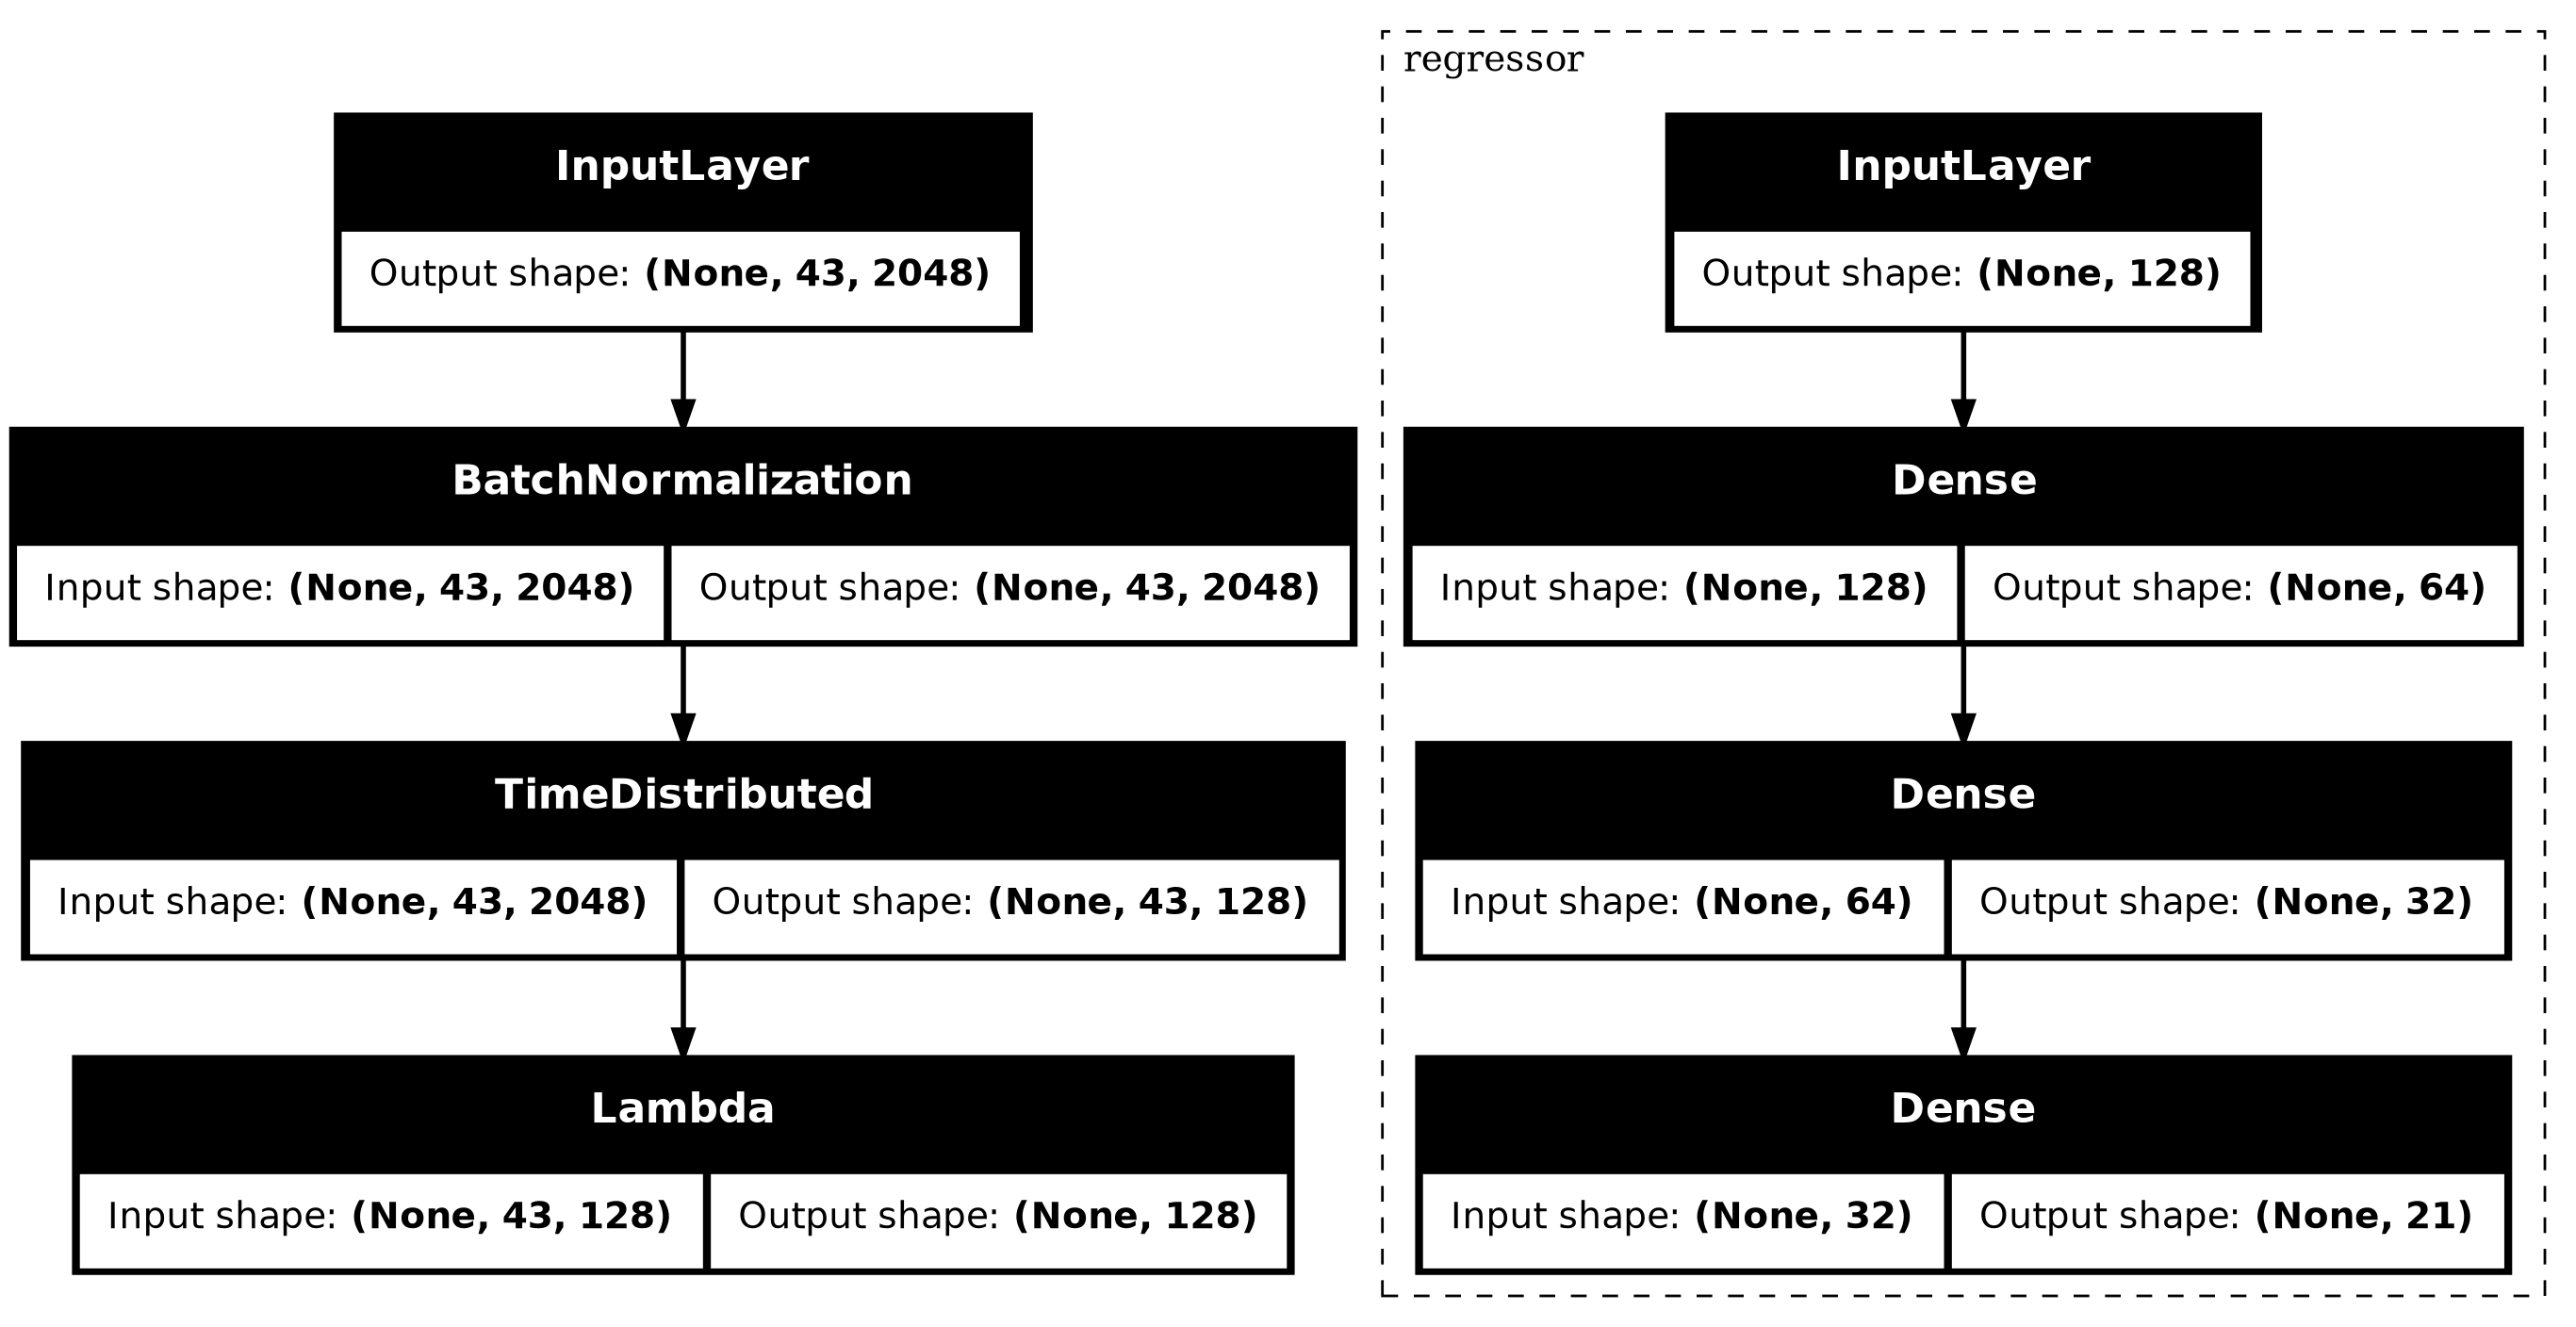
\includegraphics[scale=0.15]{images/experiment1.png}
 \fdireta{usp:logo}
\end{figure}

Summary of the evaluation metrics from the training process:

\begin{figure}[htb]
 \caption{Experiment 1 MSE error}
 \label{fig:experiment1_mse}
 \centering
 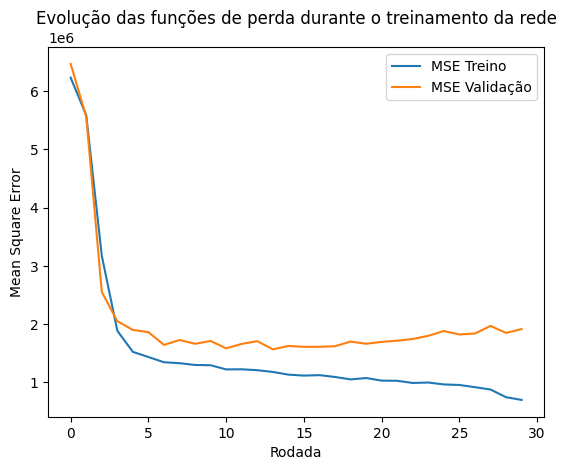
\includegraphics[scale=1]{images/experiment1_mse.png}
 \fdireta{usp:logo}
\end{figure}

\begin{figure}[htb]
 \caption{Experiment 1 MAE error}
 \label{fig:experiment1_mae}
 \centering
 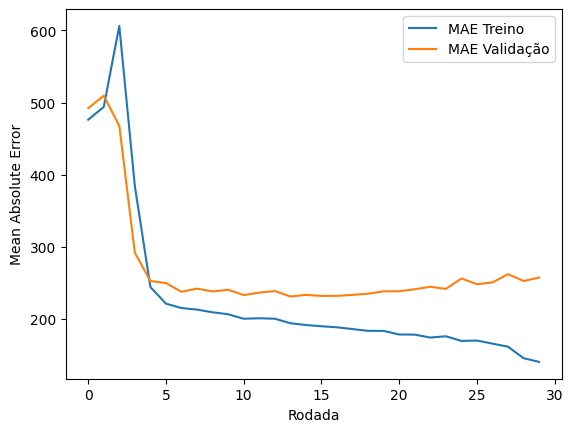
\includegraphics[scale=1]{images/experiment1_mae.png}
 \fdireta{usp:logo}
\end{figure}

\section{Experiment 2}

Use of a 1D Convolutional Neural Network to extract audio features from the time-domain representation, and to estimate the corresponding FM synthesis parameters using a standard Multilayer Neural Network. Main highlights:

\begin{enumerate}
\item 1000 audio input samples (each 1 second long, to avoid memory exhaustion).
\item The audio inputs were not further split into frames.
\item The neural network was divided into two parts: the first acted as a feature extractor, consisting of three convolutional layers; the second was a regressor, made up of a conventional neural network (with three layers) used to estimate the FM synthesis parameters based on the previously extracted audio features.
\item The results were better than in previous experiments, but still poor. Moreover, the model suffered from even more intense overfitting (despite testing many variations).
\end{enumerate}

The network architecture is presented below:

\begin{figure}[htb]
 \caption{Experiment 2 architecture}
 \label{fig:experiment2_arch}
 \centering
 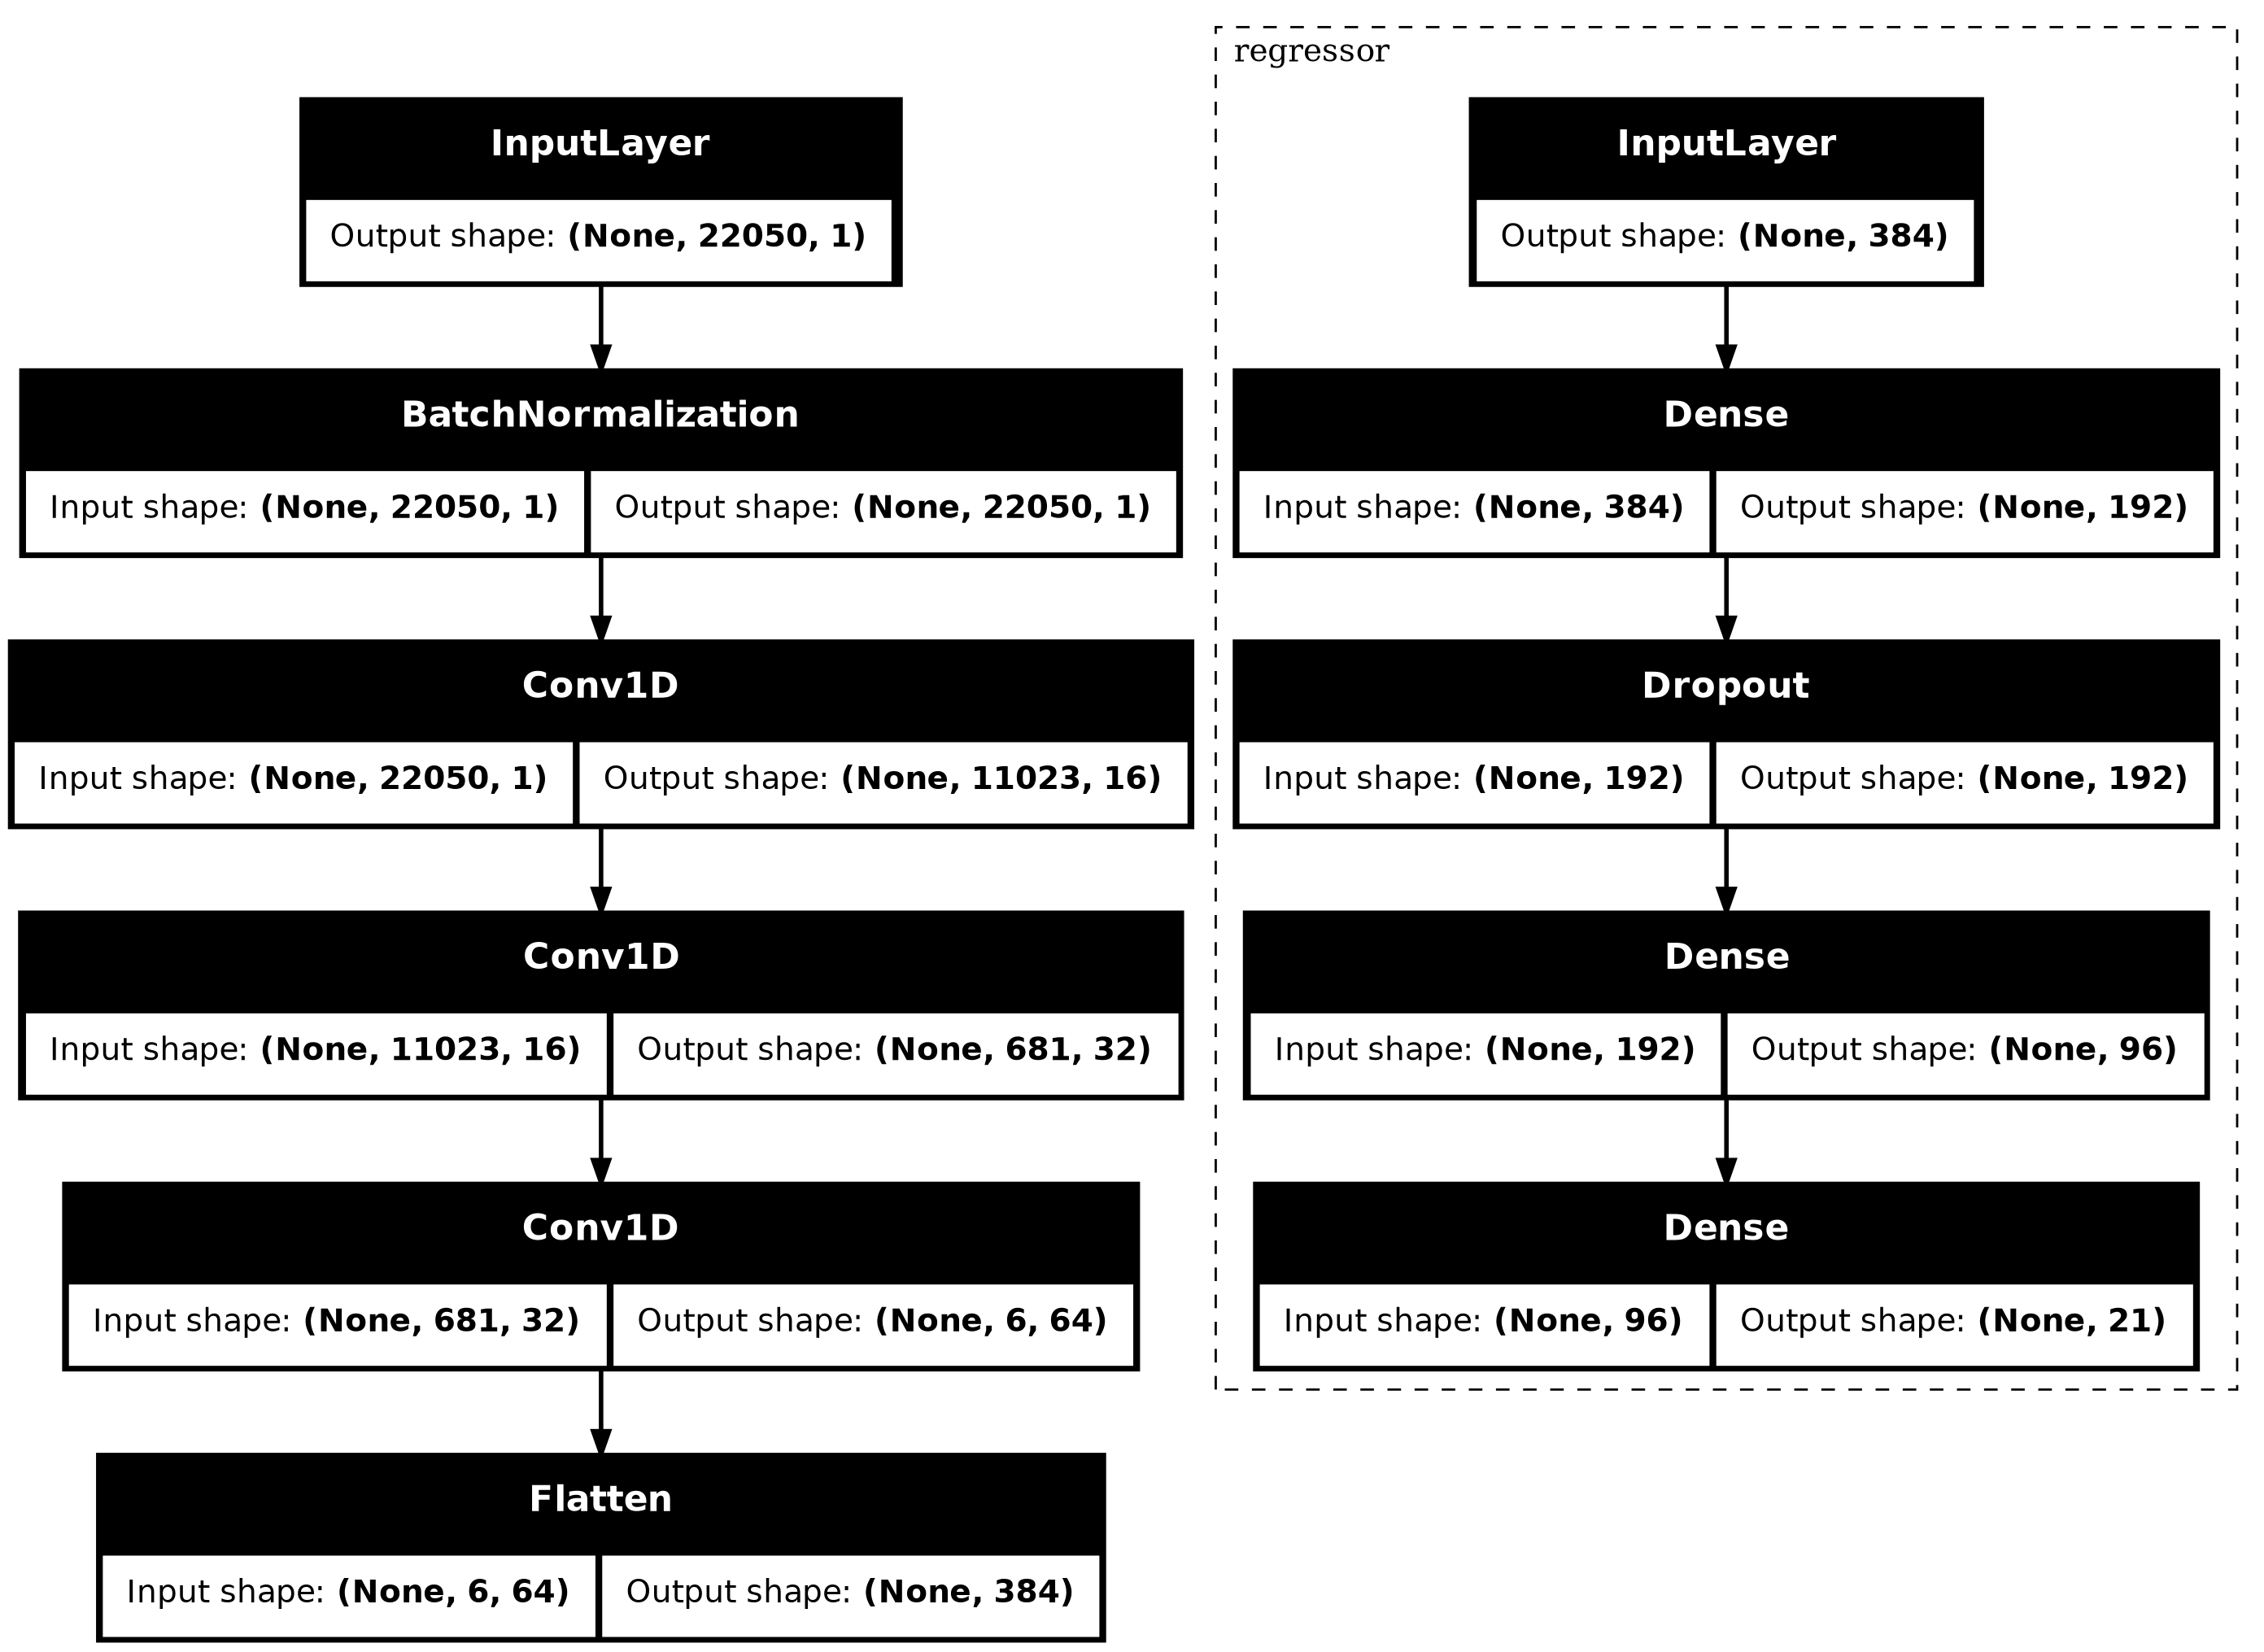
\includegraphics[scale=0.18]{images/experiment2.png}
 \fdireta{usp:logo}
\end{figure}

Summary of the evaluation metrics from the training process:

\begin{figure}[htb]
 \caption{Experiment 2 MSE error}
 \label{fig:experiment2_mse}
 \centering
 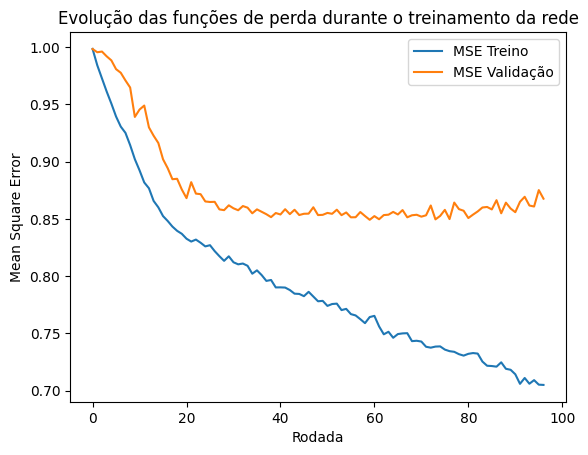
\includegraphics[scale=1]{images/experiment2_mse.png}
 \fdireta{usp:logo}
\end{figure}

\begin{figure}[htb]
 \caption{Experiment 2 MAE error}
 \label{fig:experiment2_mae}
 \centering
 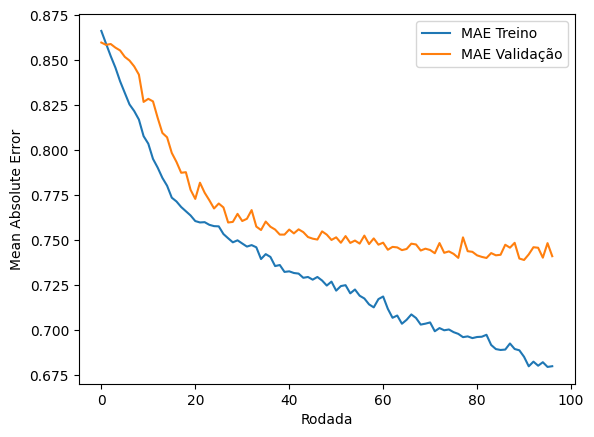
\includegraphics[scale=1]{images/experiment2_mae.png}
 \fdireta{usp:logo}
\end{figure}

\section{Experiment 3}

Very similar to the Experiment 2, but, with one convolutional layer less, but adding MaxPooling layers, on the extractor network.

\begin{enumerate}
\item 1000 audio input samples (each 1 second long, to avoid memory exhaustion).
\item The neural network was divided into two parts: the first acted as a feature extractor, consisting of three convolutional layers, plus poolgin layers; the second was a regressor, made up of a conventional neural network (with three layers) used to estimate the FM synthesis parameters based on the previously extracted audio features.
\item The results were similar to the previous experiments.
\end{enumerate}

The network architecture is presented below:

\begin{figure}[htb]
 \caption{Experiment 3 architecture}
 \label{fig:experiment3_arch}
 \centering
 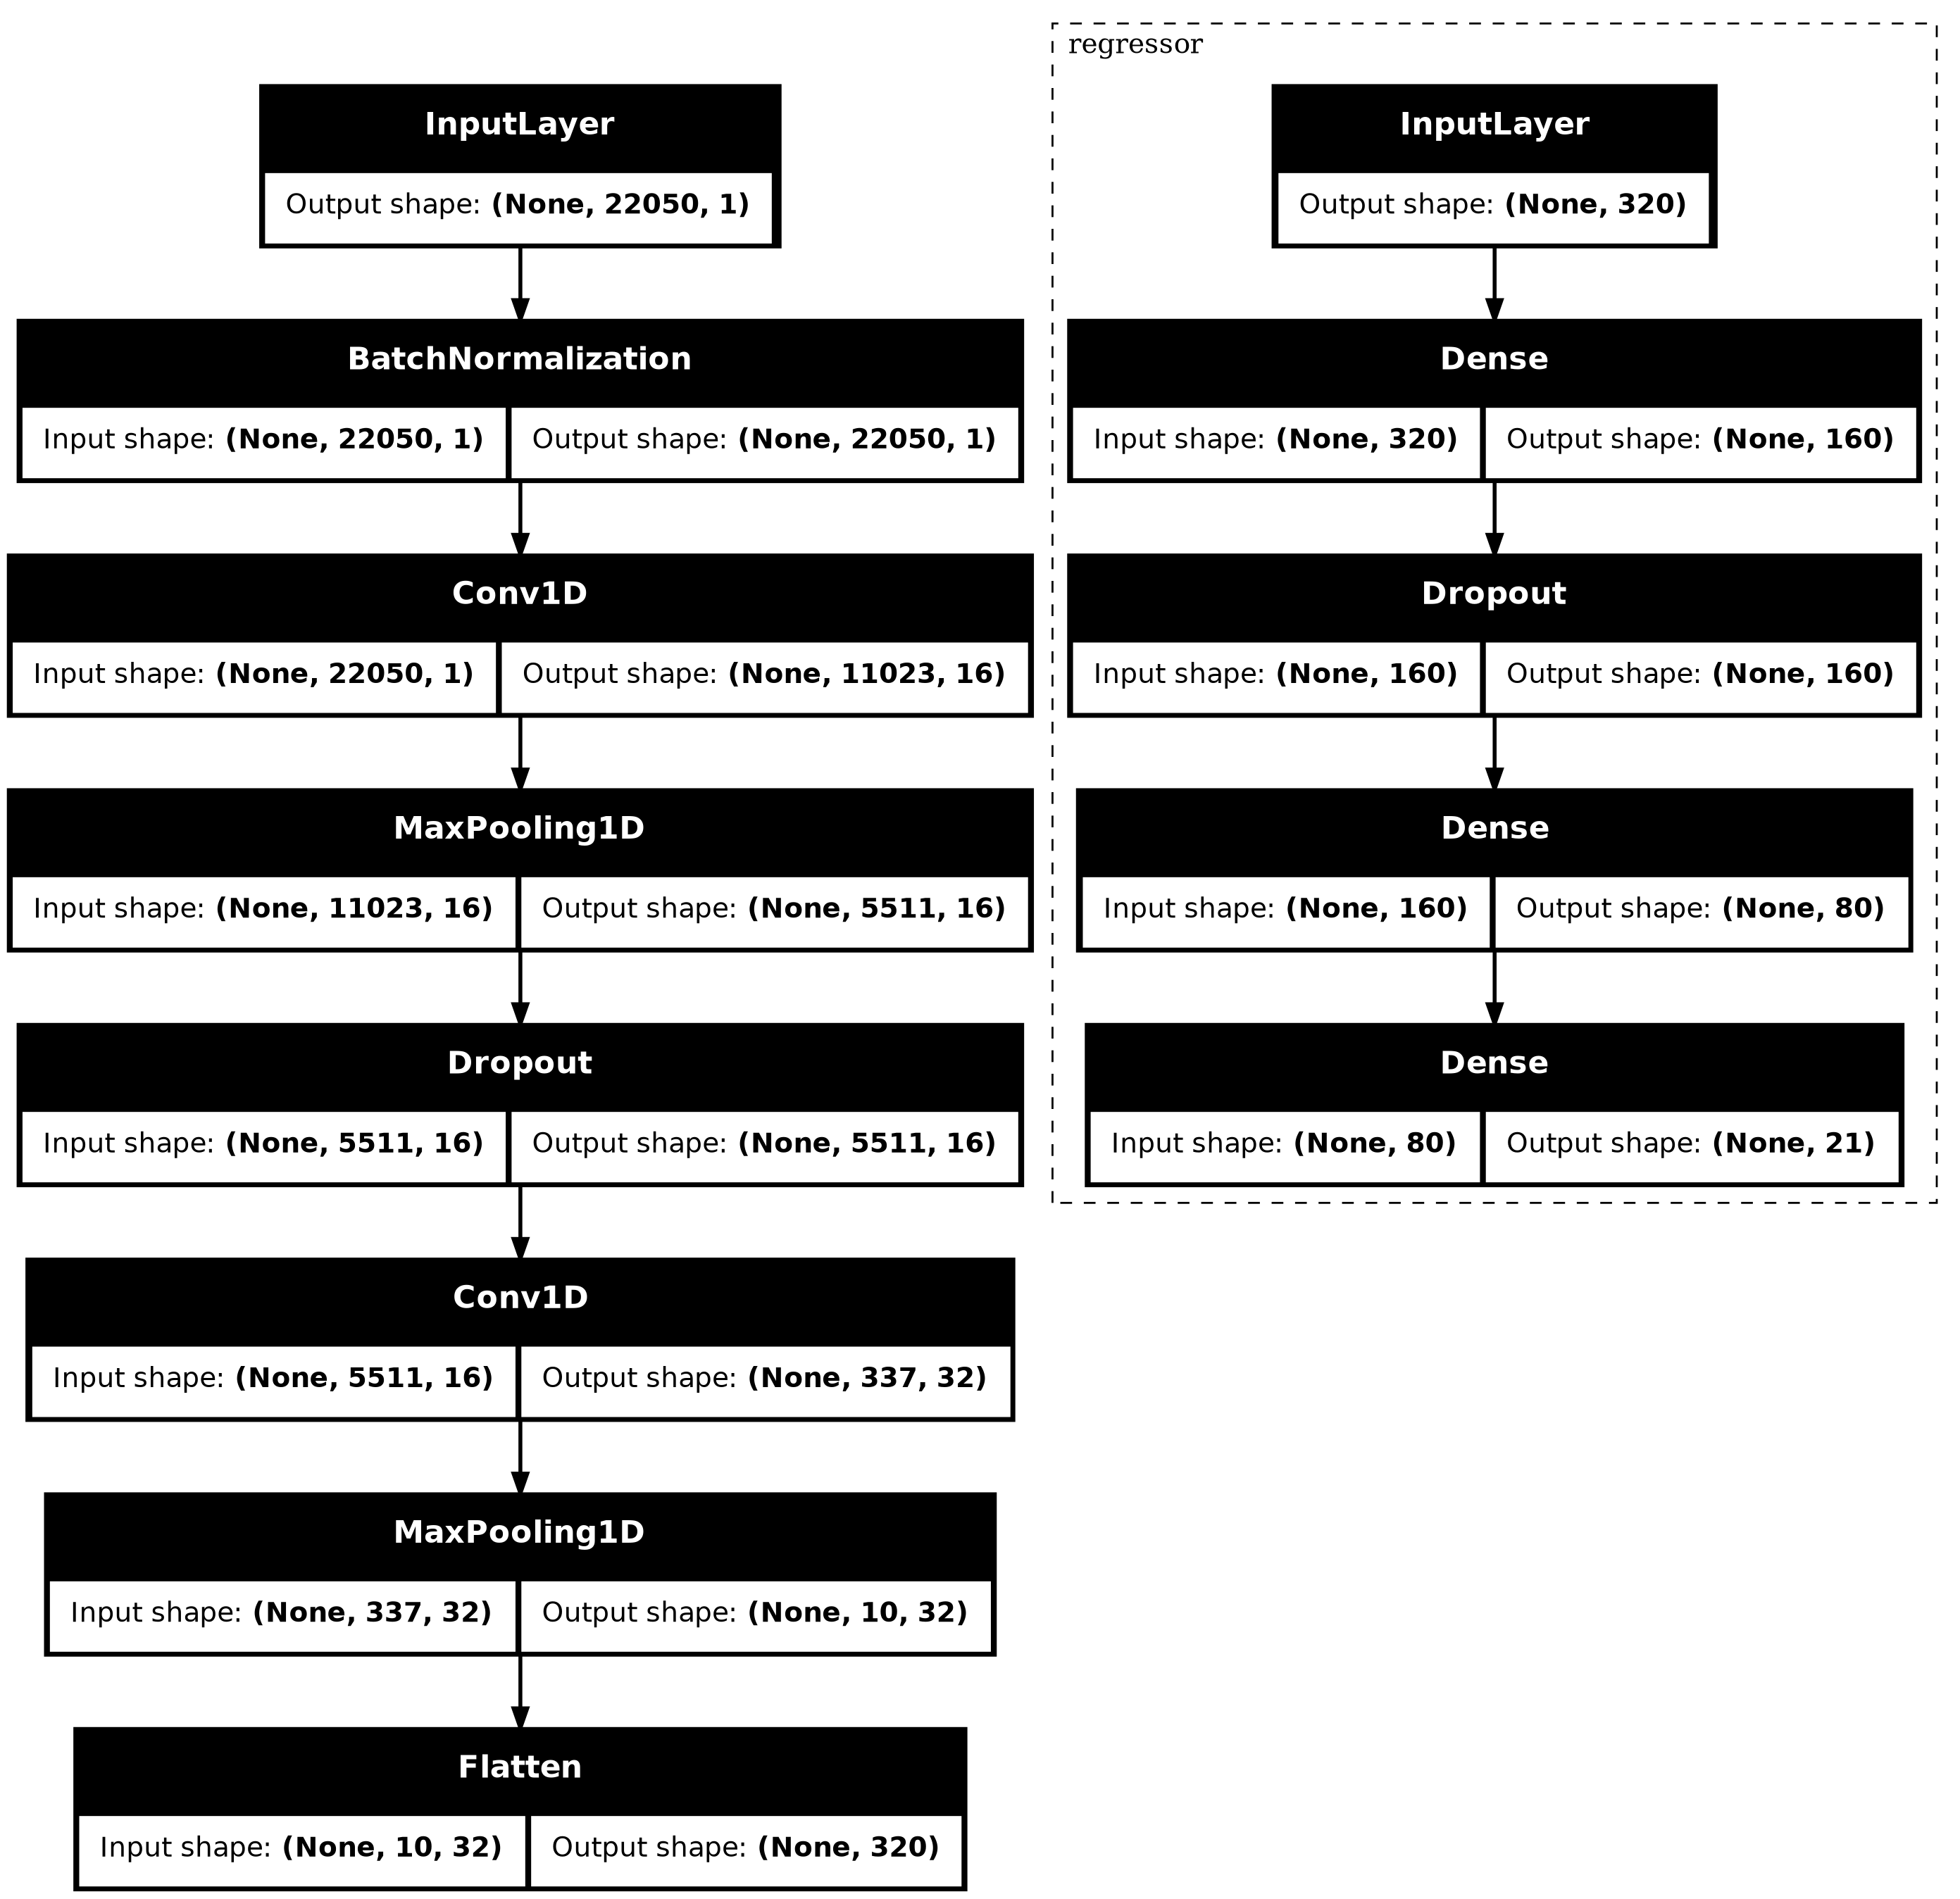
\includegraphics[scale=0.18]{images/experiment3.png}
 \fdireta{usp:logo}
\end{figure}

Summary of the evaluation metrics from the training process:

\begin{figure}[htb]
 \caption{Experiment 3 MSE error}
 \label{fig:experiment3_mse}
 \centering
 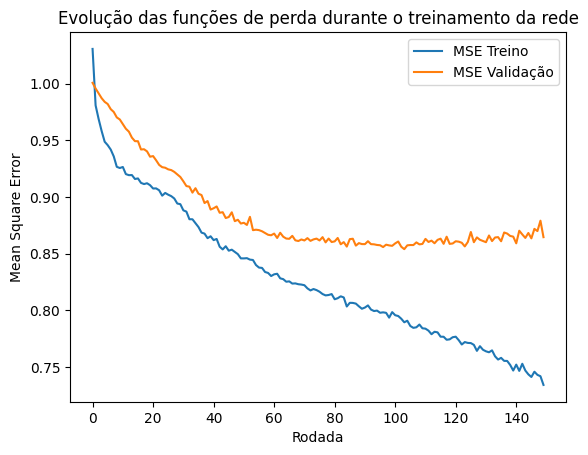
\includegraphics[scale=1]{images/experiment3_mse.png}
 \fdireta{usp:logo}
\end{figure}

\begin{figure}[htb]
 \caption{Experiment 3 MAE error}
 \label{fig:experiment3_mae}
 \centering
 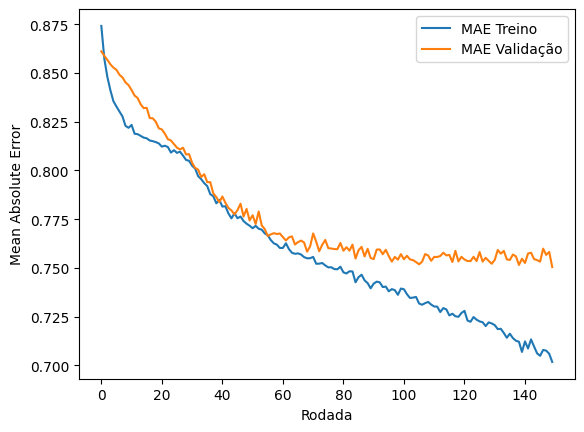
\includegraphics[scale=1]{images/experiment3_mae.png}
 \fdireta{usp:logo}
\end{figure}

\section{Experiment 4}

This experiment is very similar to Experiments 2 and 3, but with two branches of convolutional layers in the feature extraction part of the model.

Here, pooling layers are also used. The main idea is to apply different filters and pooling strategies in each branch, in order to capture distinct features and recognize different frequency patterns in the audio input.

The regression model remains similar to the previous experiments.

\begin{enumerate}
\item 1000 audio input samples (each 1 second long, to avoid memory exhaustion).
\item The neural network was divided into two main parts: a feature extractor and a regressor. However, the feature extractor itself was composed of two parallel convolutional branches.
\item The results were slightly worse than in the previous experiment, but still similar. However, this time, the model did not suffer from overfitting.
\end{enumerate}

The network architecture is presented below:

\begin{figure}[htb]
 \caption{Experiment 4 architecture}
 \label{fig:experiment4_arch}
 \centering
 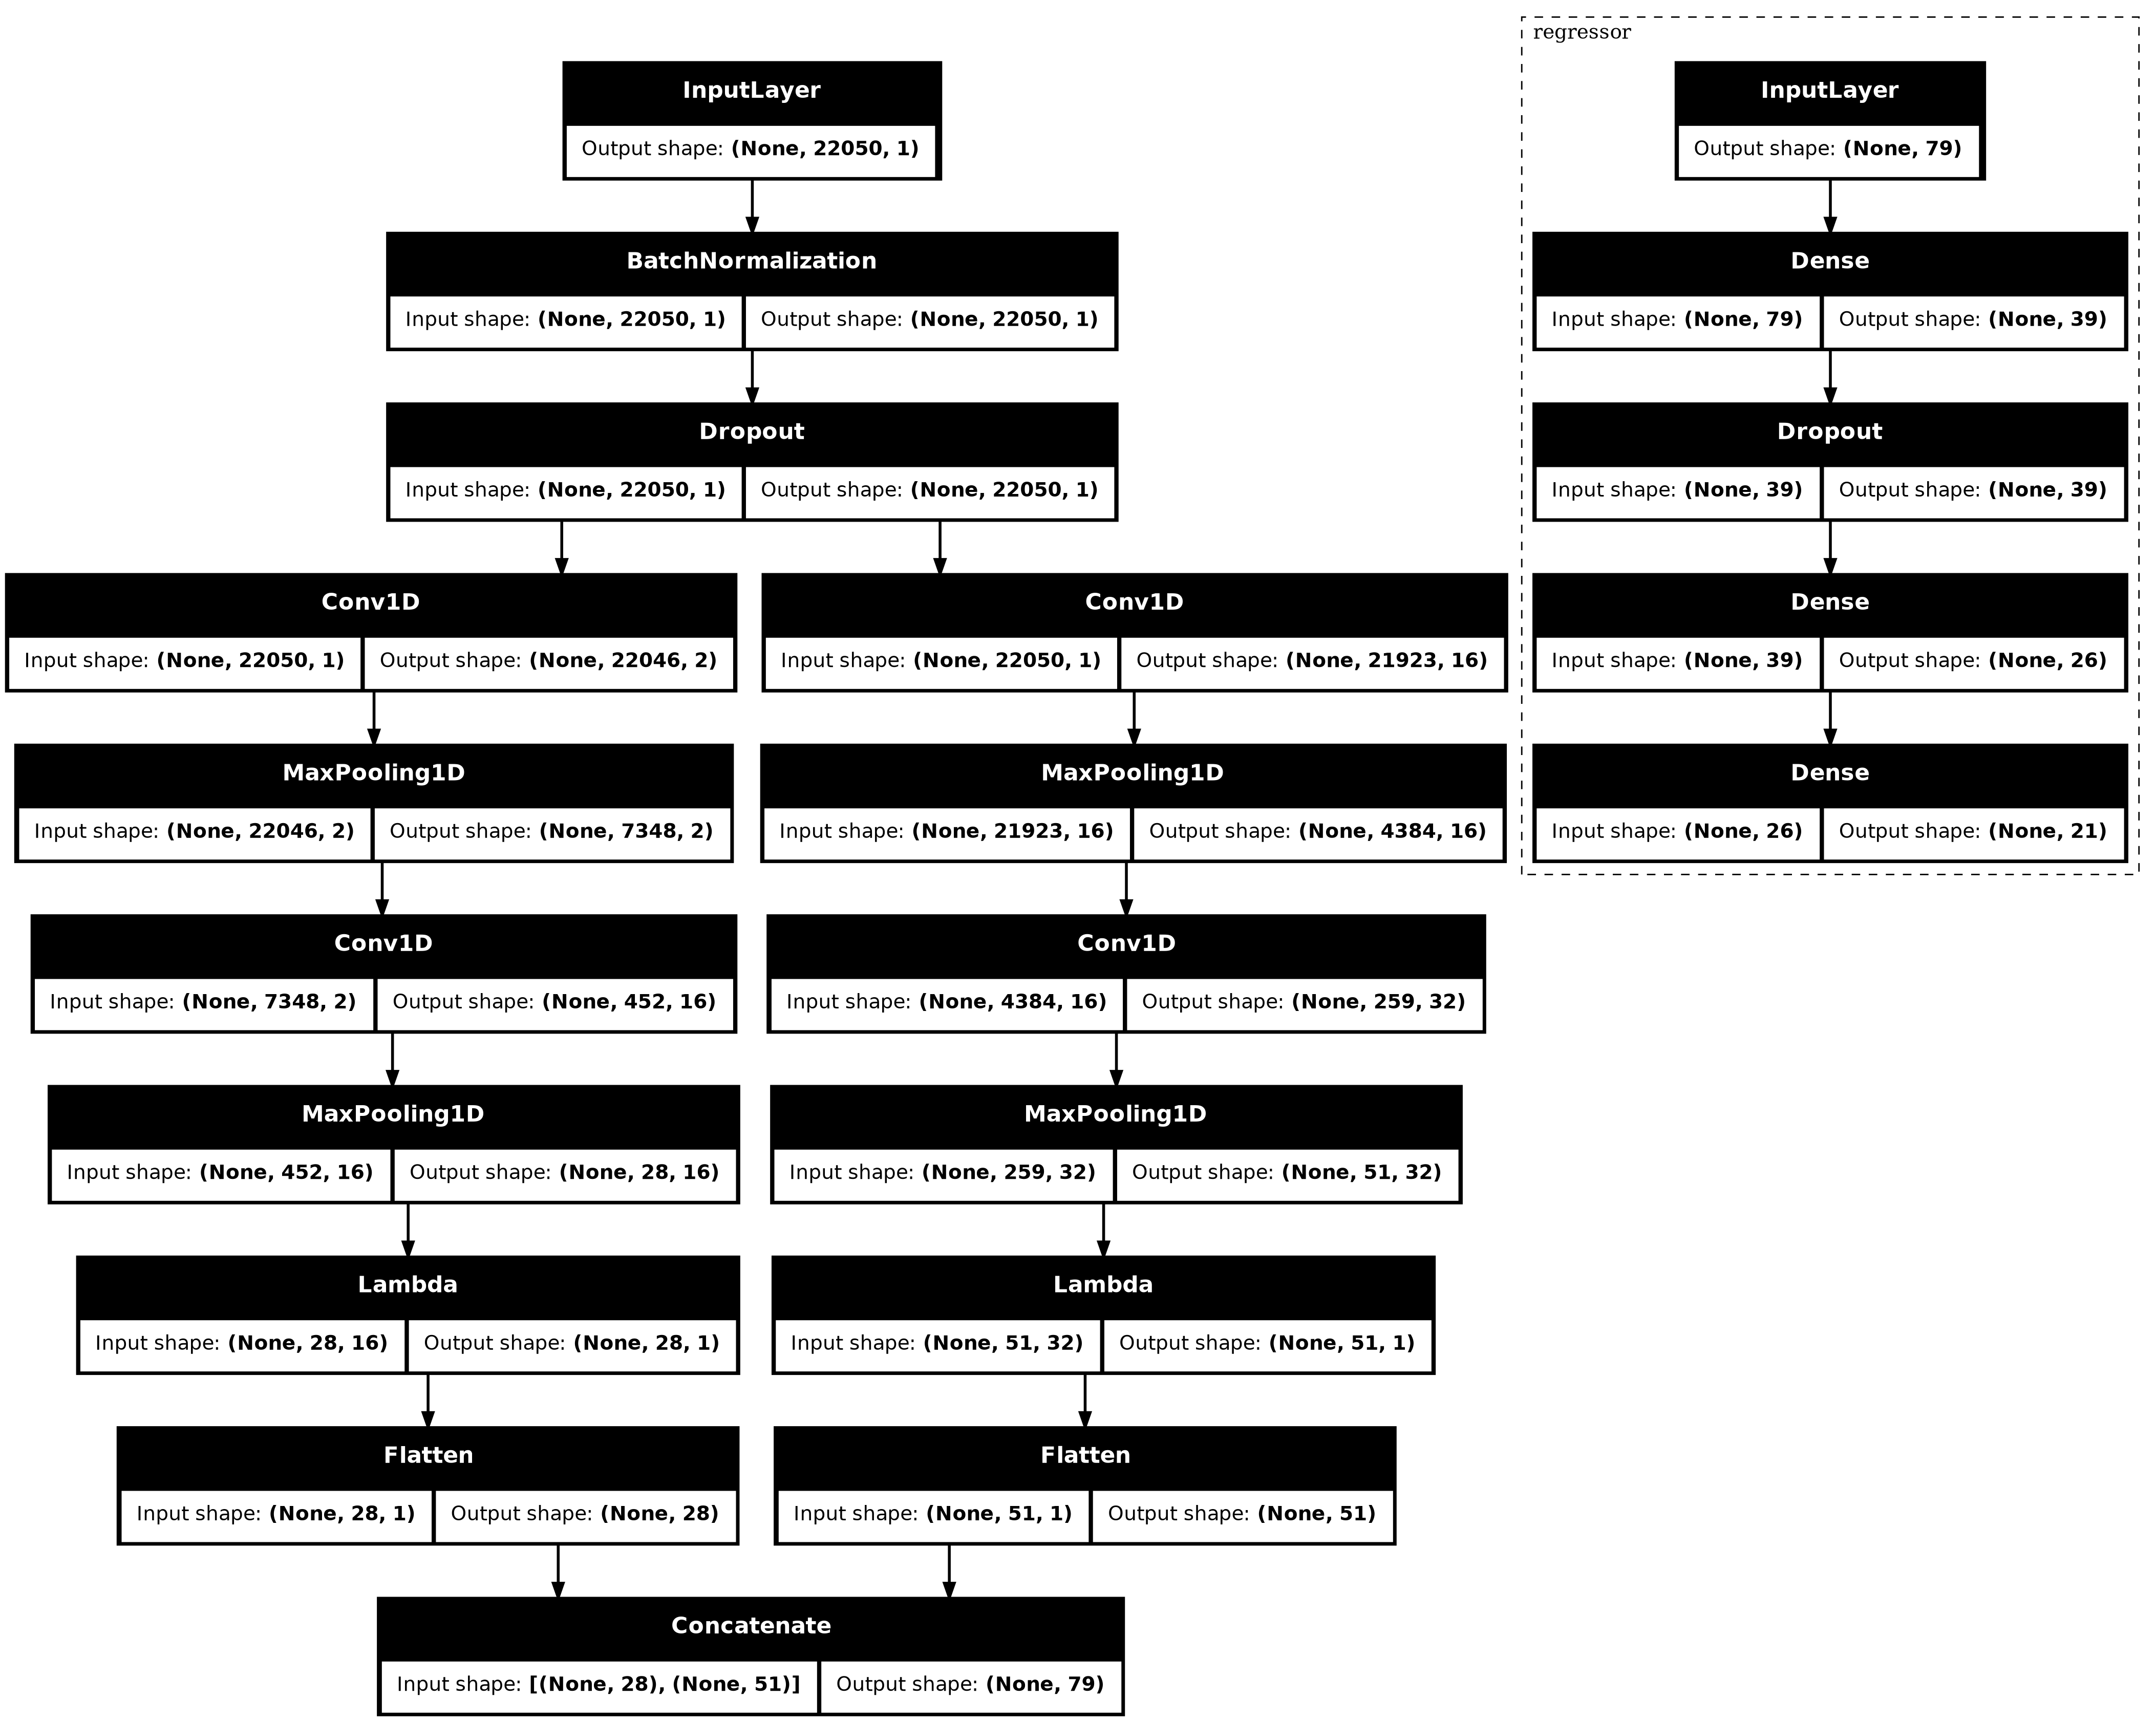
\includegraphics[scale=0.11]{images/experiment4.png}
 \fdireta{usp:logo}
\end{figure}

Summary of the evaluation metrics from the training process:

\begin{figure}[htb]
 \caption{Experiment 4 MSE error}
 \label{fig:experiment4_mse}
 \centering
 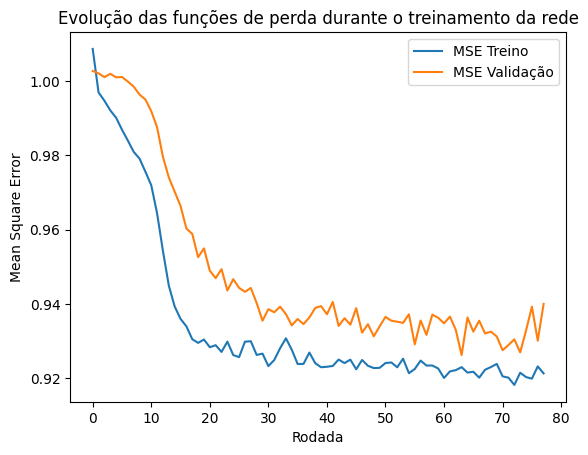
\includegraphics[scale=1]{images/experiment4_mse.png}
 \fdireta{usp:logo}
\end{figure}

\begin{figure}[htb]
 \caption{Experiment 4 MAE error}
 \label{fig:experiment4_mae}
 \centering
 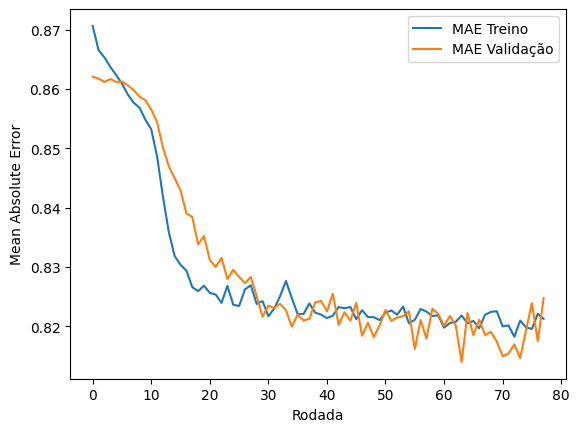
\includegraphics[scale=1]{images/experiment4_mae.png}
 \fdireta{usp:logo}
\end{figure}


\end{anexosenv}
---

\end{document}
